\chapter{Event Reconstruction}
\label{ch:EventReconstruction}

Event reconstruction is the process by which detector signals are converted into objects that can be used for physics analysis. This is a complex process that requires a great deal of focused effort by the \ac{ATLAS} collaboration. First, digital signals from the detector are collected into tracks and clusters, then they are combined to form reconstruction-level physics objects. Then, a identification steps is performed, where quality requirements are placed on the reconstruction-level objects to identify them as signatures of physical particles, like electrons and muons, that can be used in physics analyses. 

These algorithms are centrally developed by the collaboration and are generally designed to reconstruct and identify prompt objects ($|d_{0}| < 10 \textrm{mm}$). This section describes this process for objects which are relevant to this analysis, as well as the changes to these algorithms that have been implemented to be able to study objects with a wider range in \dzero.  

Reconstruction of tracks, including modifications to reconstruct tracks with high impact parameter, is described in \autoref{sec:trackreco}. Electron and muon reconstruction, as well as their modifications, are described in \autoref{sec:elecreco} and \autoref{sec:muonreco}, respectively. The reconstruction of jets, photons, and $\tau$ leptons is not discussed here. All of these objects are reconstructed in this analysis, though no selection is made on them. 


%-----------------------------
% Track Reconstruction
%-----------------------------
\section{Track Reconstruction}
\label{sec:trackreco}

Track reconstruction is the process by which \ac{ID} data is converted into particle trajectories. This is a complicated process, due to both the density of each event in the detector (in Run 2, there were an average of 40 collisons per bunch crossing, all of which produce hadronic sprays of particles), as well the helical trajectory (in $\phi$) the particles take due to the solenoidal magnetic field. Tracks are described by five parameters with respect to the beamspot position: \dzero (the transverse point of closest approach, or transverse impact parameter), \zzero (the longitudinal point of closest approach, or longitudinal impact parameter), $\phi$ (the azimuthal angle of the track momentum), $\theta$ (the polar angle of the track momentum), and $q/p$ (the ratio of the track's charge to the magnitude of its momentum). \cite{track-algo}


%From ATLAS-tracking-algo.pdf
First, clusters from the \ac{ID} are converted into three-dimensional \emph{space-points}. In the Pixel detector, a space-point is simply one cluster, while in the \ac{SCT}, it is taken from both sides of a strip layer.

%From ATLAS-LRT.pdf
Tracking in ATLAS is performed in two steps. During the first step, called \emph{inside-out}, tracks are seeded from the silicon layers. In the Pixel and \ac{SCT} detectors, track seeds are formed from sets of three space-points, each from a separate silicon layer. If the seed passes an assortment of selection criteria, including on the \pt and \dzero, track candidates are built using a combinatorial Kalman filter (further described in \autoref{sec:kalman}). Seed requirements serve to cut down on the number of times the computationally expensive Kalman filter must be run. Multiple track candidates can be built from the same seed.

%From ATLAS-tracking-algo.pdf
Since all possible track combinations are created in the previous stage, an \emph{ambiguity solving} step is now required. Tracks are scored based on a variety of criteria, the number of holes (detector elements the track could have intersected with, but do not contain a cluster), $\chi^{2}$ (to prioritize tracks with a better fit), and \pt (to prioritize tracks with a higher \pt). A further requirement that no more than two tracks may share the same cluster reduces the number of duplicate tracks; however, a cluster may be removed from a track to stay within this limit and the track is then re-scored. 

Next, the track candidates are extended into the  \ac{TRT} using a classical track extrapolation technique, then the track is scored using a method similar to the ambiguity solver. If this extension is successful, the track is labeled as having a \emph{\ac{TRT} extension}, though the track can still be retained if this extensin fails, particularly at large $|\eta|$. However, if the score after TRT extension is worse than the silicon-only score, the track is rejected. This completes the \emph{inside-out} step.

\comebackto{How does classical extrapolation work?}


Step two takes an \emph{outside-in} approach, where track segments are reconstructed in the \ac{TRT}, seeded by deposits in the \ac{EM} calorimeter. These segments are then extended inward to the silicon detectors, where any clusters not used in step one can be associated to the track. The extension inward is not required, as \ac{TRT}-only tracks are used for reconstructing and identifying converted photons. 


\subsection{Large Radius Tracking}

\ac{LRT} \cite{lrt} is required to reconstruct tracks with impact parameters larger than what is allowed by the \ac{ST} algorithm. These requirements are designed for a maximum displacement a few mm, to enable the identification of heavy flavor hadron decays.

An optional third step of the tracking chain, it uses the same \emph{inside-out} tracking algorithm, but relaxes various requirements that allow for a much more inclusive track collection. The major changes are summarized in \autoref{tab:LRT}. These cuts are applied during both the seeding and extension steps. Additionally, \ac{LRT} uses a sequential Kalman filter as opposed to the combinatorial Kalman filter used in \ac{ST}.

\ac{LRT} is required for this analysis, but cannot be applied to all events in the Run 2 dataset. The full event reconstruction with \ac{LRT} takes about 2.5 times longer than with \ac{ST}, so events are filtered based on the triggers that selected them, such that this algorithm is only run on about 10\% of the dataset.


\begin{table}
\centering
\begin{tabular}{lcc}
Cut & \ac{ST} & \ac{LRT}  \\
\hline
$d_{0}^{\textrm{max}}$ (mm)   & 10   & 300 \\
$z_{0}^{\textrm{max}}$ (mm)   & 250   & 1500 \\
$ |\eta^{\textrm{max}}|$        & 2.7   & 5 \\
Max shared silicon modules    & 1     & 2 \\
Min unshared silicon clusters   & 6     & 5 \\
Min number of silicon hits   & 7     & 7 \\
\hline
\end{tabular}
\caption{Most important cuts that differ between \ac{ST} and \ac{LRT}}
\label{tab:LRT}
\end{table}

\begin{figure}[htbp]
\centering
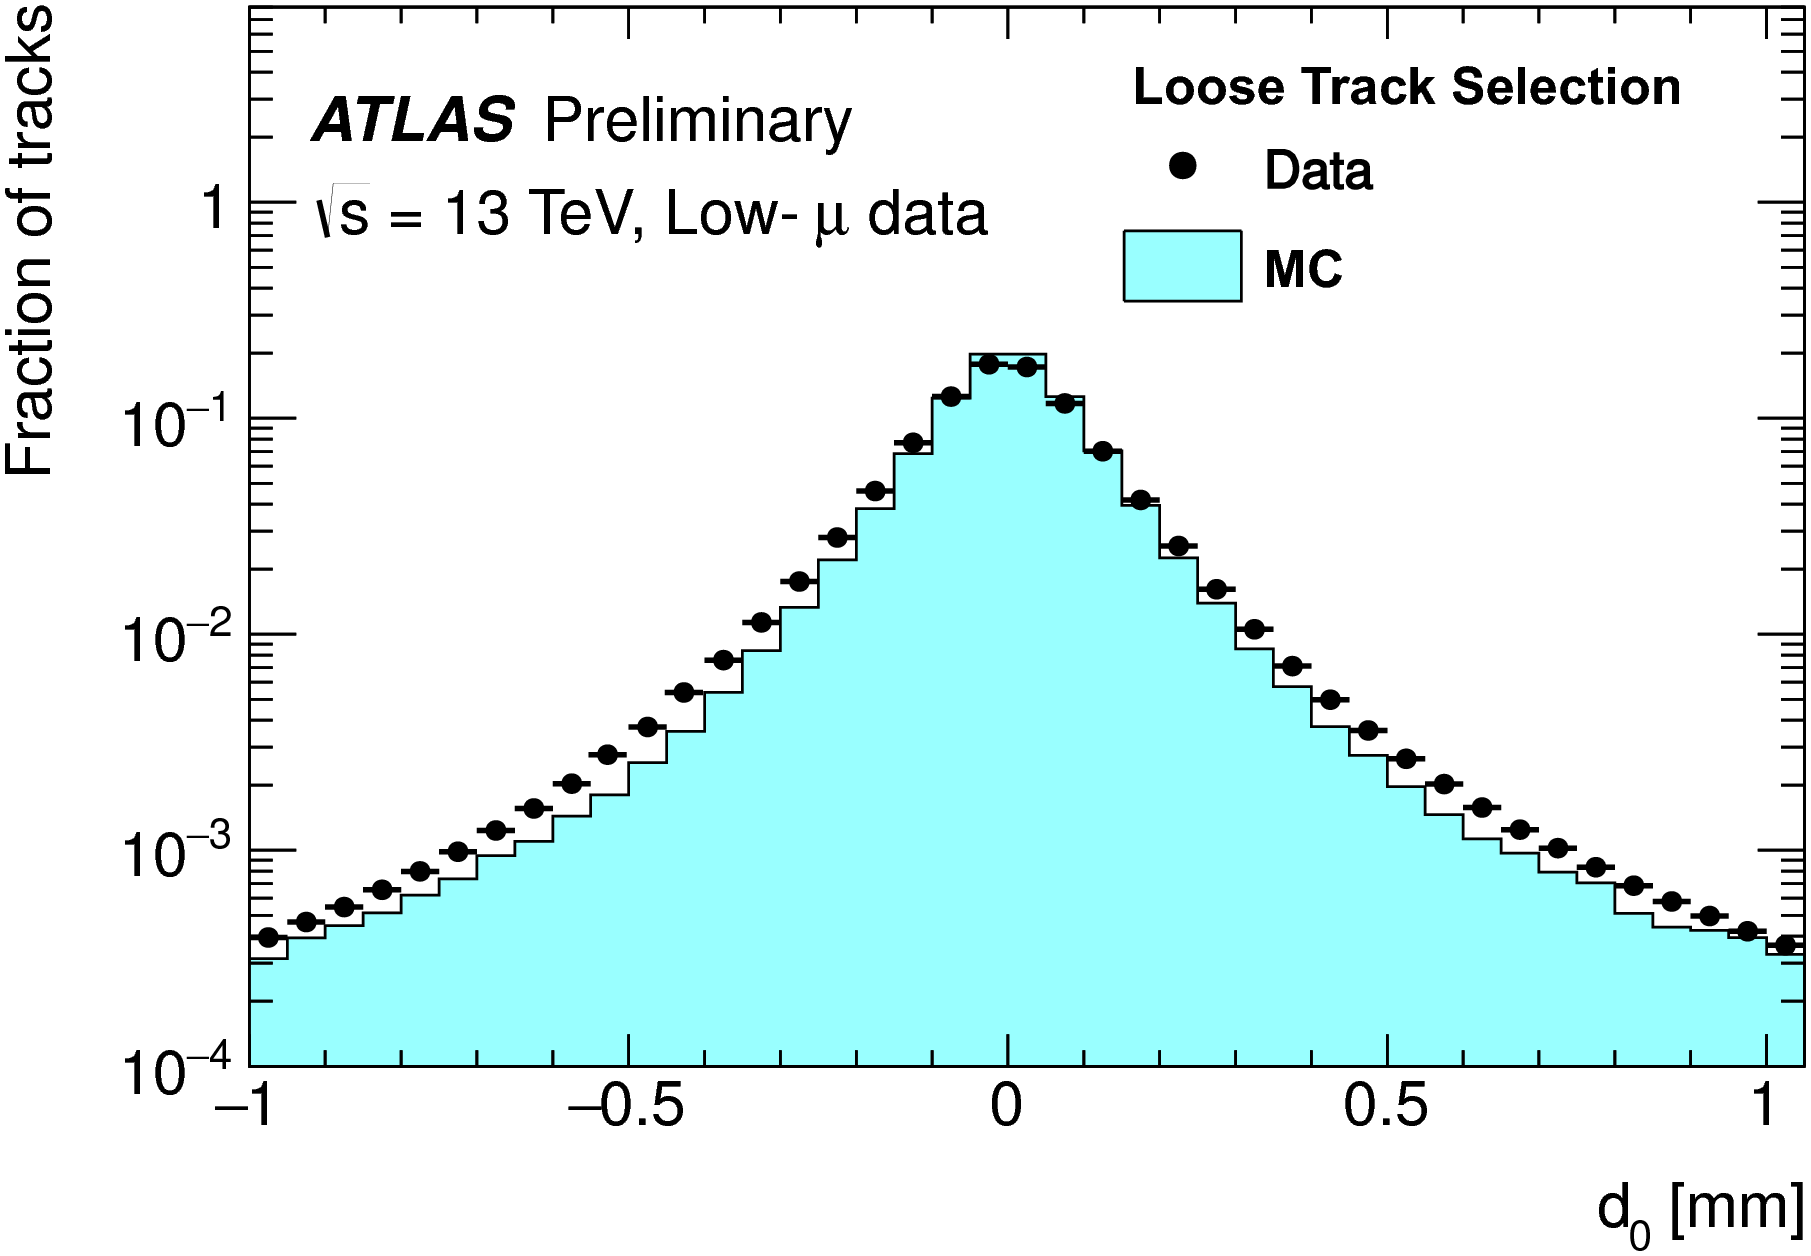
\includegraphics[width=.5\textwidth]{figures/EventReconstruction/ST-d0-eff.png}
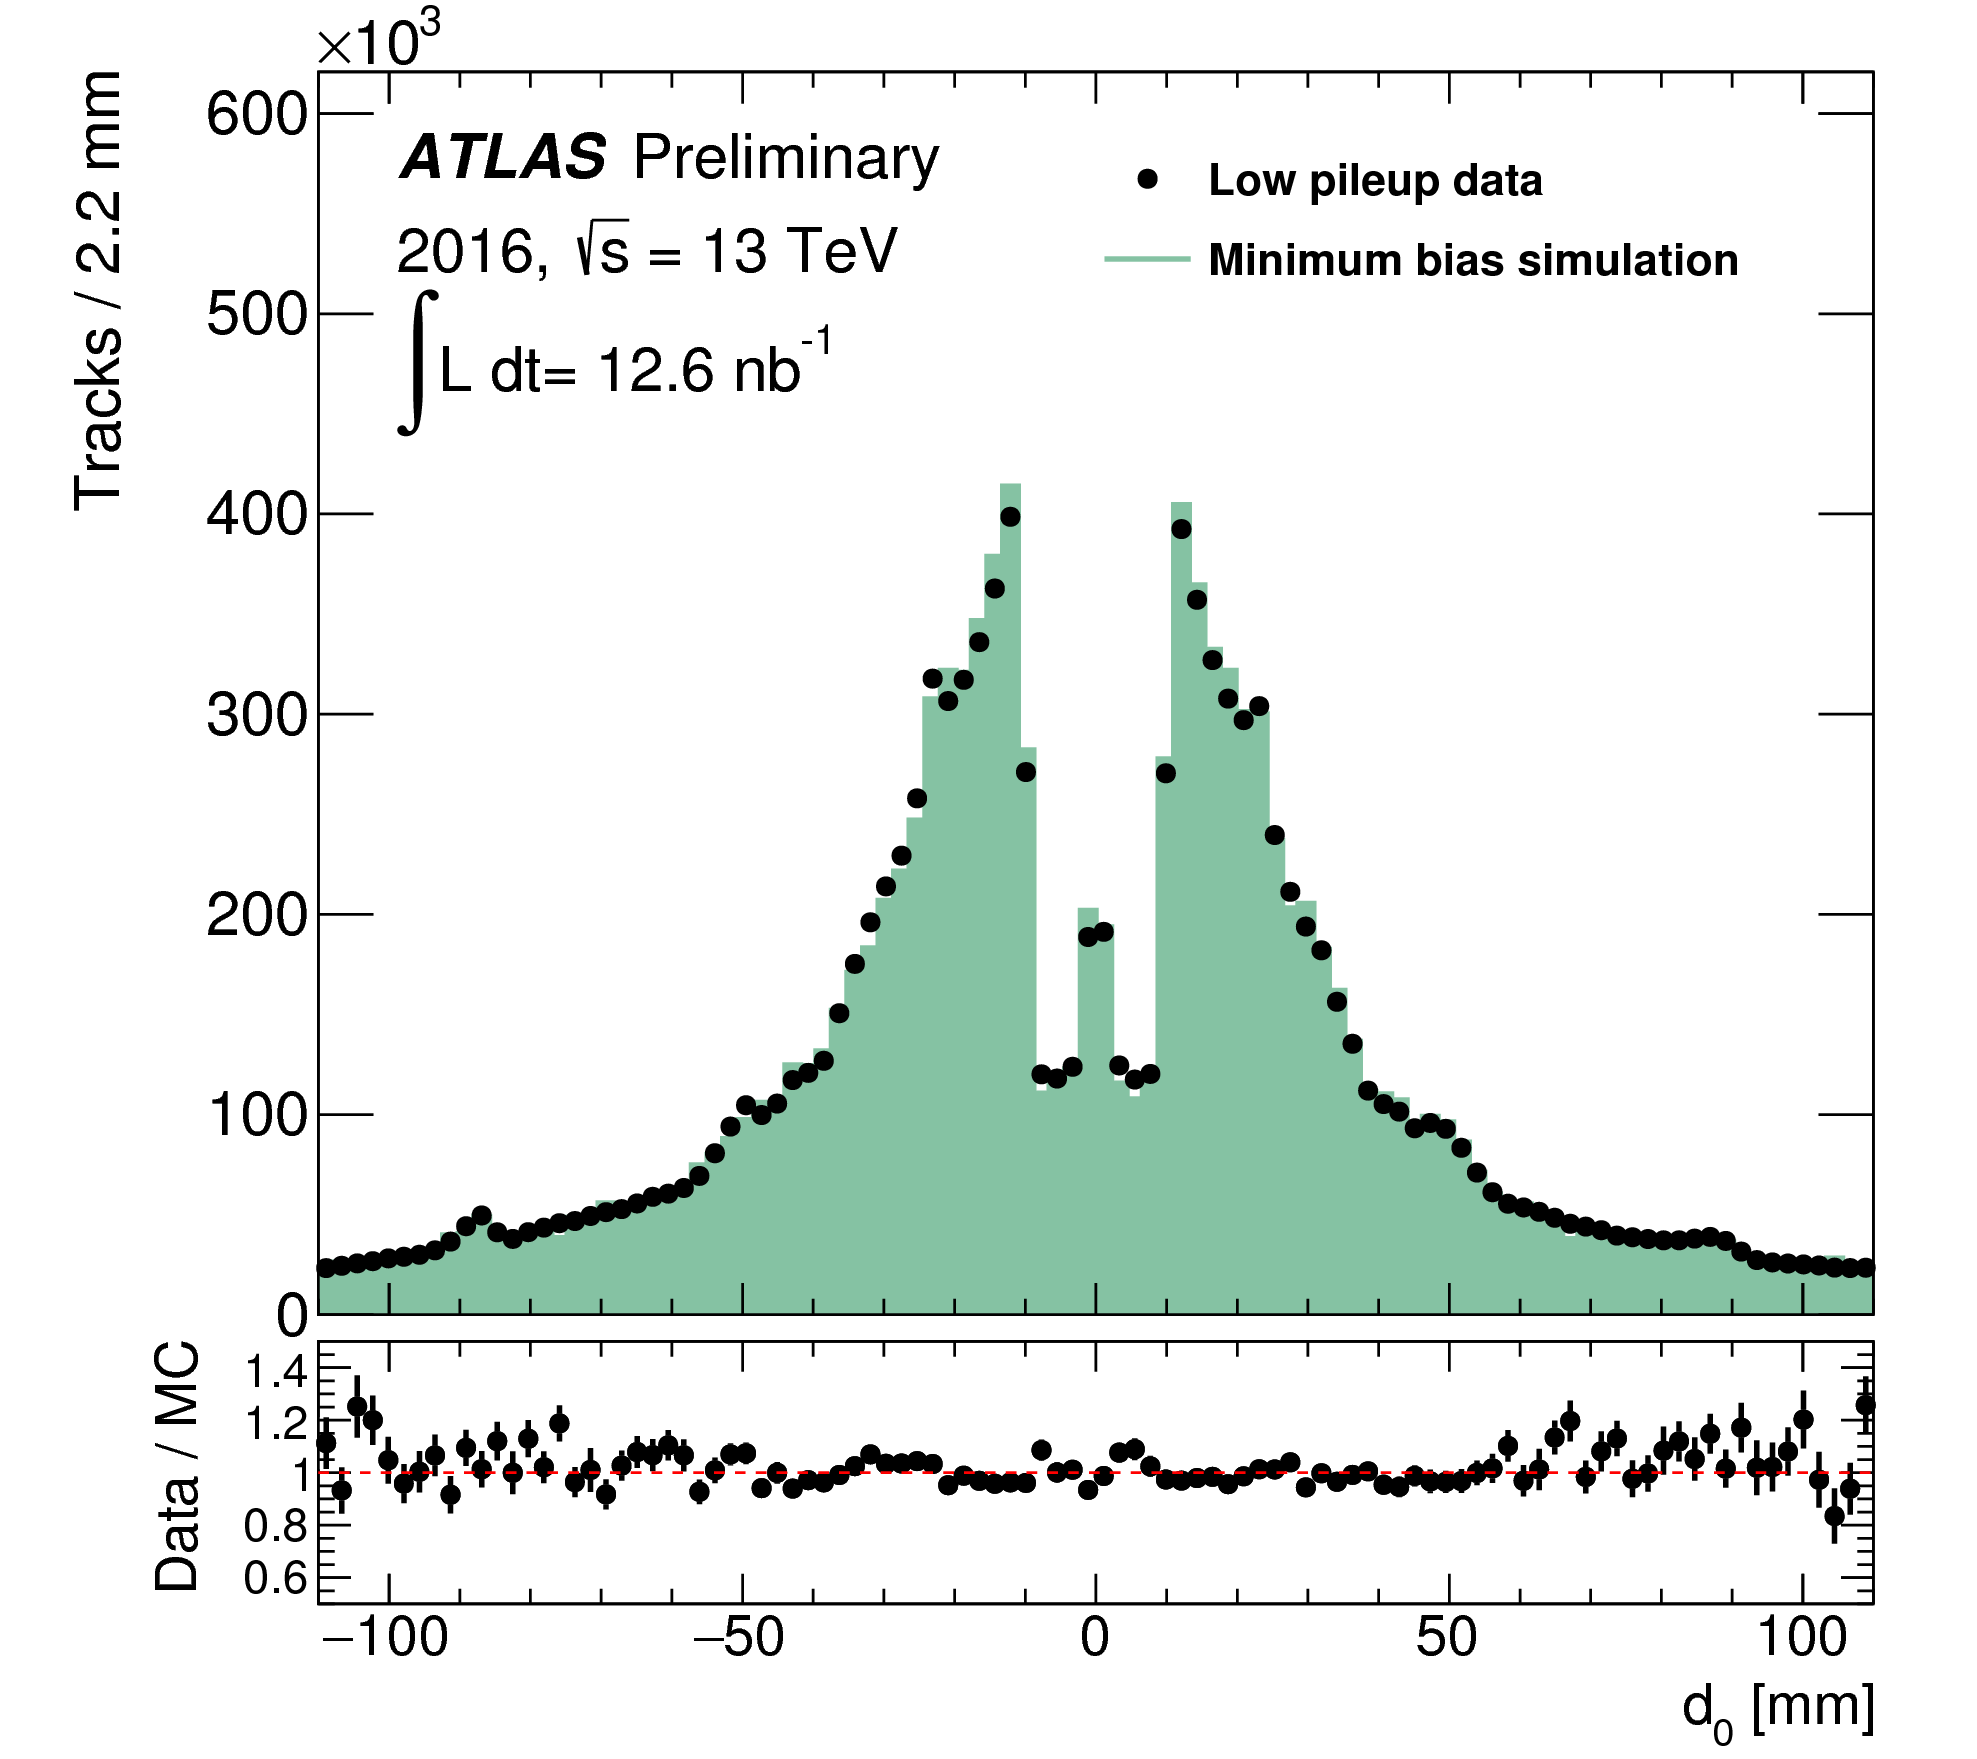
\includegraphics[width=.41\textwidth]{figures/EventReconstruction/LRT-d0-eff.png}
\caption{Number of tracks reconstructed with respect to \dzero in \ac{ST} (left) and \ac{LRT}. Note the difference in x-axis range.}
\label{fig:trking_d0_eff}
\end{figure}

\begin{figure}[htbp]
\centering
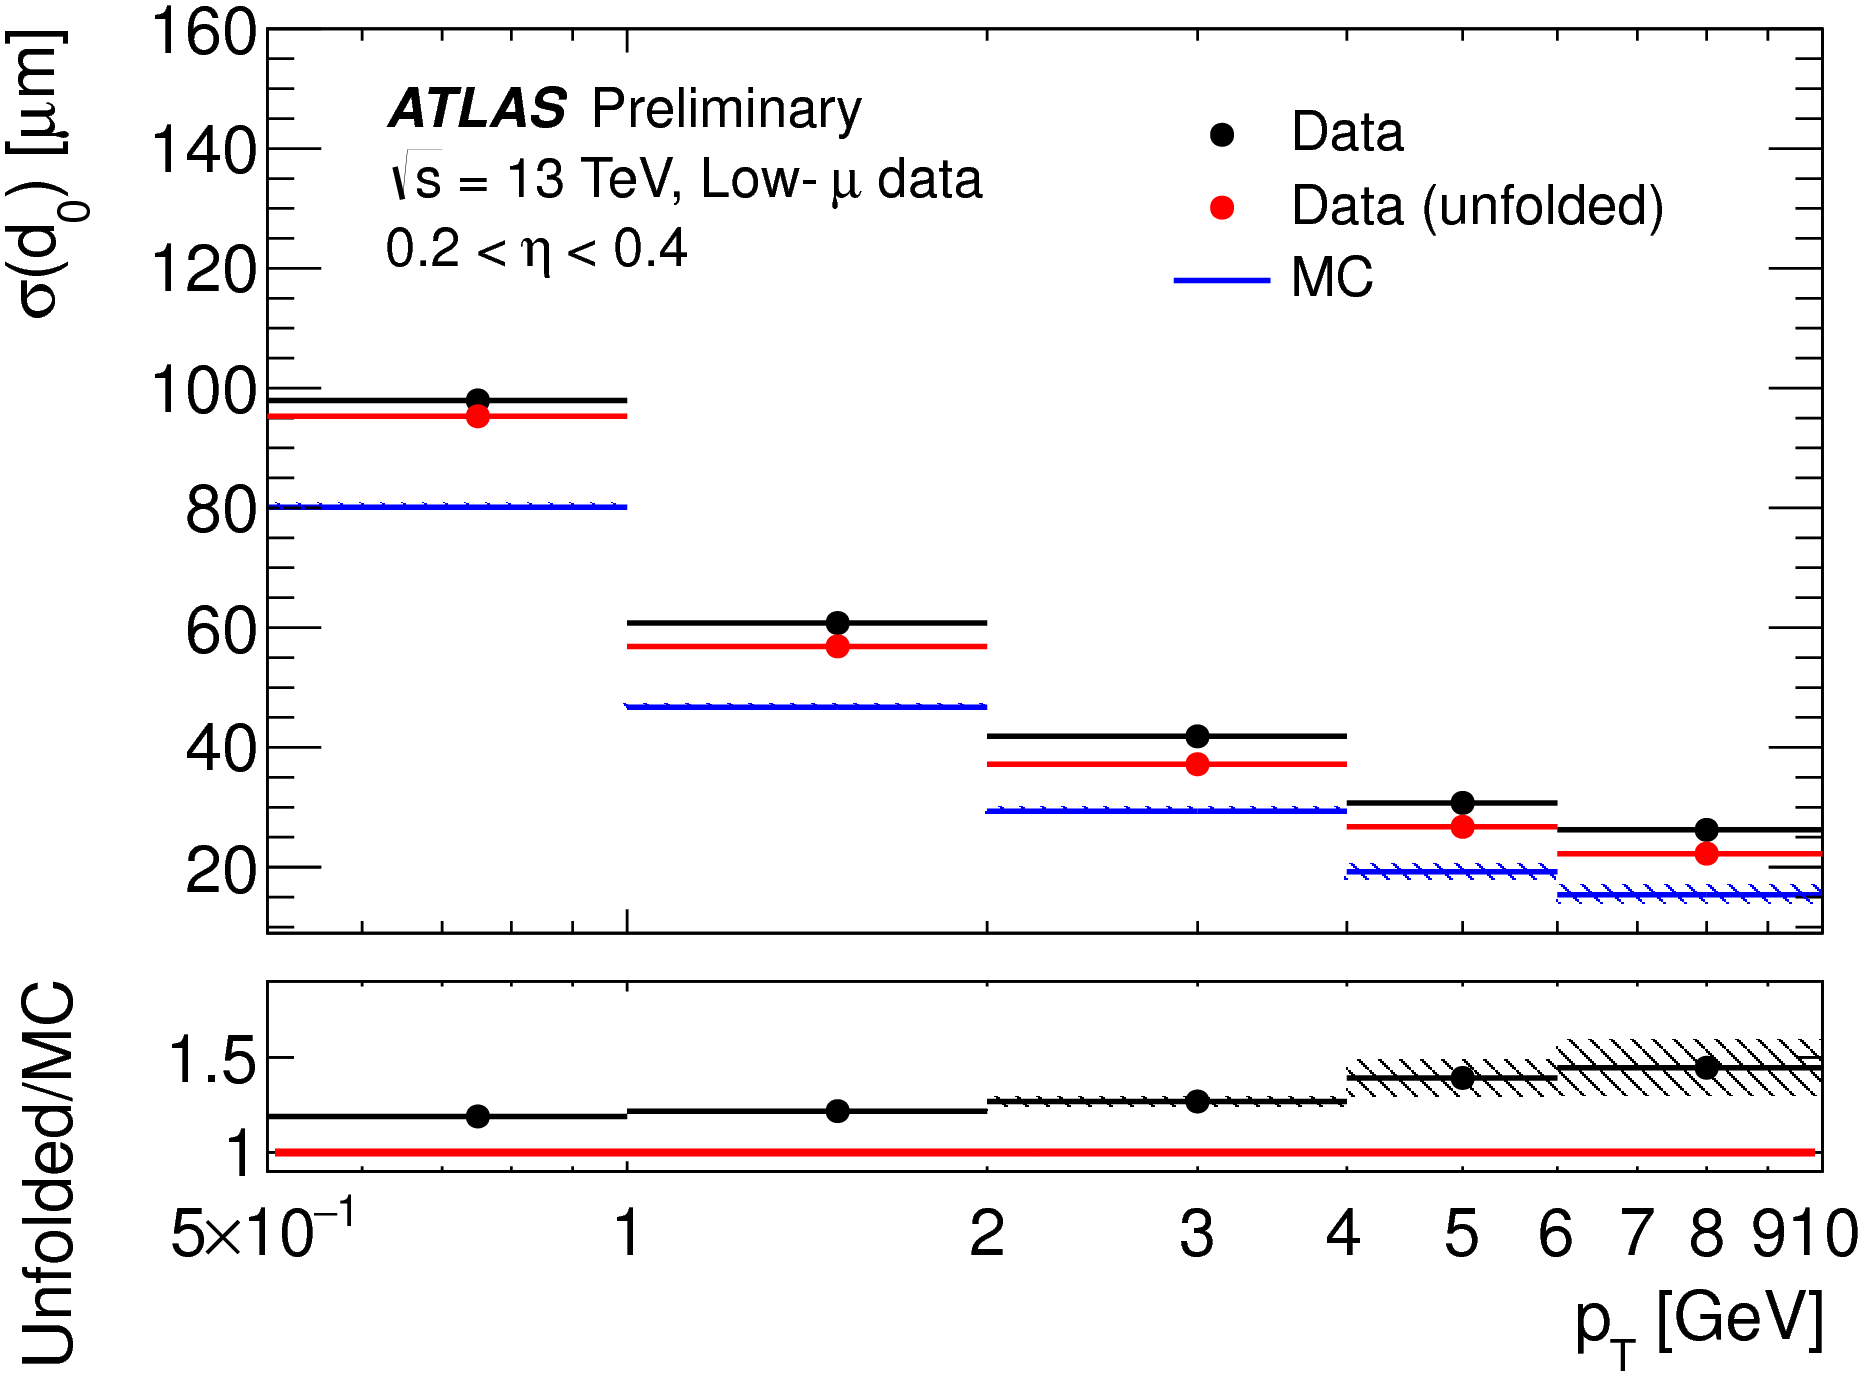
\includegraphics[width=.45\textwidth]{figures/EventReconstruction/ST-d0-res.png}
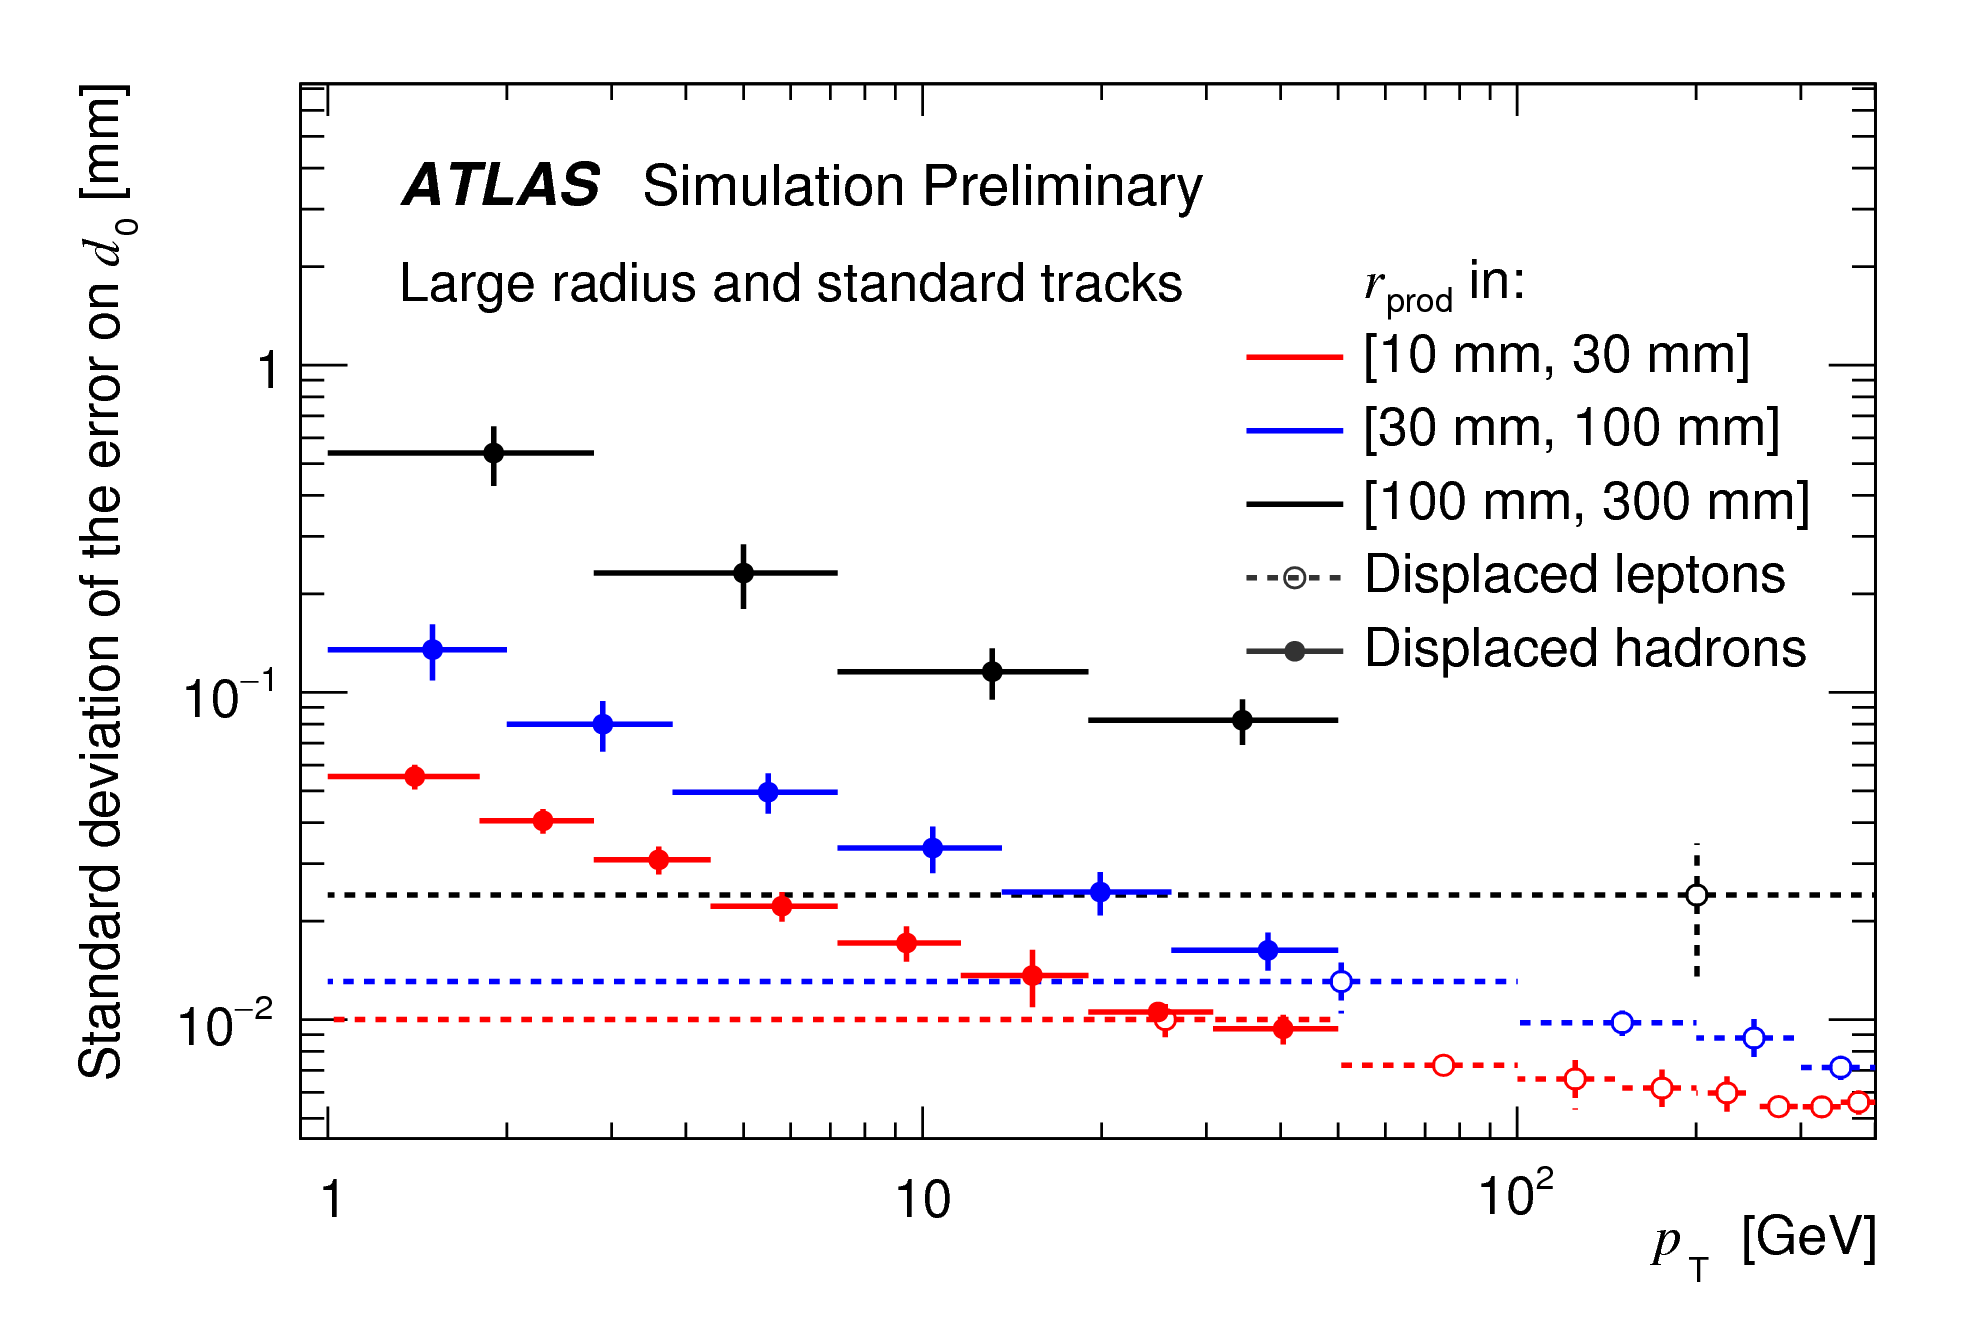
\includegraphics[width=.5\textwidth]{figures/EventReconstruction/LRT-d0-res.png}
\caption{\dzero resolution as a function of \pt in \ac{ST} (left) and \ac{LRT}. This analysis uses high \pt leptons with high \pt tracks, and thus with very good \dzero resolution}
\label{fig:trking_d0_res}
\end{figure}

%mostly used this: https://pdfs.semanticscholar.org/a591/7c383e4b07d64116b57c9c33e82138a08d12.pdf (p19+)
\subsection{Tracking Algorithms}

\subsubsection{\label{sec:kalman} Kalman Filter}

Kalman filters are widely used across LHC experiments for track fitting. It is a recursive algorithm that allows the user to efficiently extrapolate from a track seed. In the sequential, or extended, Kalman filter, uses a linear approximation to the track path. It makes a prediction for the next layer of detector material based on the seed, and then looks for a hit in that region. At each step, it updates the linearization to improve the measurement for the next step, where each measurement is weighted by its certainty. \ac{LRT} uses this approach.

In \ac{ST}, a combinatorial Kalman filter is used. This method employs several Kalman filters running in parallel and allows for the assumption that the measurement in the next layer is not necessarily assumed to be part of the track that formed the seed (as is often the case in the dense environment of the \ac{ATLAS} \ac{ID}). At each successive layer in track finding, several branches are extended if several measurements can be found in the same layer. The update of the linearization is done independently for each branch, and branches are created for missing measurements to account for detector inefficiencies. The branch is extended to the next layer if a measurement is found, and the process is repeated. Branches with no measurement for several layers are removed, and at the end, the branch with the best quality is selected. This process allows for parallelization of a complex combinatorial process. \cite{kalman-filter} 

The Kalman filter works well for tracking in environments such as \ac{ATLAS} because even though it is computationally intensive, it generally gives the best precision.

\subsubsection{\label{sec:hough} Hough Transform}

%https://indico.cern.ch/event/602049/contributions/2429704/attachments/1440531/2217489/Piucci_05_04_2017.pdf
%hough-transform.pdf

A Hough transform is a pattern recognition algorithm that is useful for identifying a particular signature that can be described in a known parametric form. It performs well in noisy environments and is tolerant of holes in the signature. In relies on a transformation from physical to parameter space. Each point in physical space maps to a line in parameter space, and the intersection of the parameter space lines gives the values of constants of the parametric form. 

For example, if the pattern being searched for is a line described by $y = mx + b$, a Hough transform maps from $x-y$ space to $m-b$ space. Each point $(x_i, y_i)$ in the original image maps to a line in parameter space. If all $(x_i, y_i)$ are plotted together, the intersections of the lines in parameter space at $(m_i, b_i)$ define lines in physical space with parameters $m_i$ and $b_i$. \cite{hough-transform}

The Hough transform is a \emph{pattern finding} algorithm, not a tracking algorithm. Is not ideal for full \ac{ID} tracking, because its complexity grows exponentially with the number of dimensions and the form of the pattern must be known \emph{a priori}.

\comebackto{How are seeds formed? Hough transform?}


\subsection{Primary Vertex Reconstruction}

After all of the tracks are reconstructed, they must be correctly assigned to a \ac{PV}. A \ac{PV} is the point in space where the $pp$ collision occurred. Generally, there are many \ac{PV}s per event: one is the hard-scatter, high-energy event of interest, and the others are pileup. In the Run 2 dataset, there are an average of 33 \ac{PV}s per event.

\ac{PV}s are reconstructed using an n iterative vertexing procedure. First, good quality tracks tracks, combined with the beamspot measurement, are used to find an optimal vertex position. Then each track is assigned a weight based on its compatibility with that position, and the vertex position is then recomputed using the weights of the tracks. After the final vertex position is determined, tracks very incompatible with the vertex are removed from it and can be used to create another vertex. Any vertex with at least two tracks are considered \ac{PV}s.



%-----------------------------
% Muon Reconstruction
%-----------------------------
\section{Muons}
%USED atlas-muon-reco.pdf
\label{sec:muonreco}
\subsection{Standard Reconstruction and Identification}

Muons are reconstructed by combining a \ac{MS} track with an \ac{ID} track. Then, at the identification stage, quality requirements are imposed on the combined tracks to improve the purity of the muon collection. For this analysis, the muon reconstruction algorithm remains unchanged (though \ac{LRT} tracks are used), while changes are made at the identification stage. \cite{muon-reco}

\subsubsection{Muon Track Reconstruction}
To reconstruct \ac{MS} tracks, a Hough transform (described in \autoref{sec:hough}) is used to search for hits in each \ac{MDT} chamber to find hits following a trajectory on the $\eta$ plane of the detector. These hits are fit to a straight line within each chamber to form \emph{segments}. Co-located \ac{RPC} and \ac{TGC} hits are used to measure the $\phi$ coordinate. 

Hits from segments in various layers are fit to form track candidates. This fitting is first seeded from segments in the middle layers of the \ac{MS} where more trigger hits are available, then extrapolated inward and outward. A next pass is done using inner and outer station segments as seeds. The extrapolation relies on relative positional and angular information, as well as the fit quality and hit multiplicity of the segments. Two segments are required to make a track, except in regions with limited detector coverage, where one high quality segment is sufficient. After all extrapolation, an overlap removal procedure is performed, allowing for a segment to be shared between at most two tracks. A $\chi^{2}$ test is performed, where outliers hits can be removed from the track and additional hits consistent with the track candidate's trajectory can be added.

\comebackto{what are "trigger hits"}


\subsubsection{Combined Muons}
Next, the \ac{MS} tracks are combined with \ac{ID} tracks to form \ac{CB} muons, a track fit over the two tracks. \ac{CB} muon tracks are generally seeded from the \ac{MS}, then extrapolated inward and matched to an \ac{ID} track, but the inverse is also allowed. Hits from the \ac{MS} may be added or removed to improve the fit between the two tracks.



\subsubsection{Muon Identification}

This analysis uses the default muon working point for ATLAS analyses, called a \emph{medium} muon. This working point places a requirement on the number of \ac{ID} and \ac{MS} hits that comprise the track to ensure a robust momentum measurement. At least 1 pixel hit, at least 5 \ac{SCT} hits are required and at least 10\% of the \ac{TRT} hits associated to the object must be included in the final fit. There must also be fewer than 3 holes in the silicon tracking layers. Furthermore, the \ac{MS} track must have at least 3 hits in at least 2 \ac{MDT} layers. In the crack region $|\eta| < 0.1$, \ac{MS} tracks with at least three hits in only one \ac{MDT} layer are allowed provided there are no holes in the track. Finally, a loose requirement is placed on the consistency between the \ac{MS} and \ac{ID} tracks. Namely, the \emph{q/p significance}, the difference between the charge and momentum ratio in the \ac{ID} and \ac{MS} divided by their uncertainties summed in quadrature, is required to be less than 7. 


\begin{figure}[htbp]
\centering
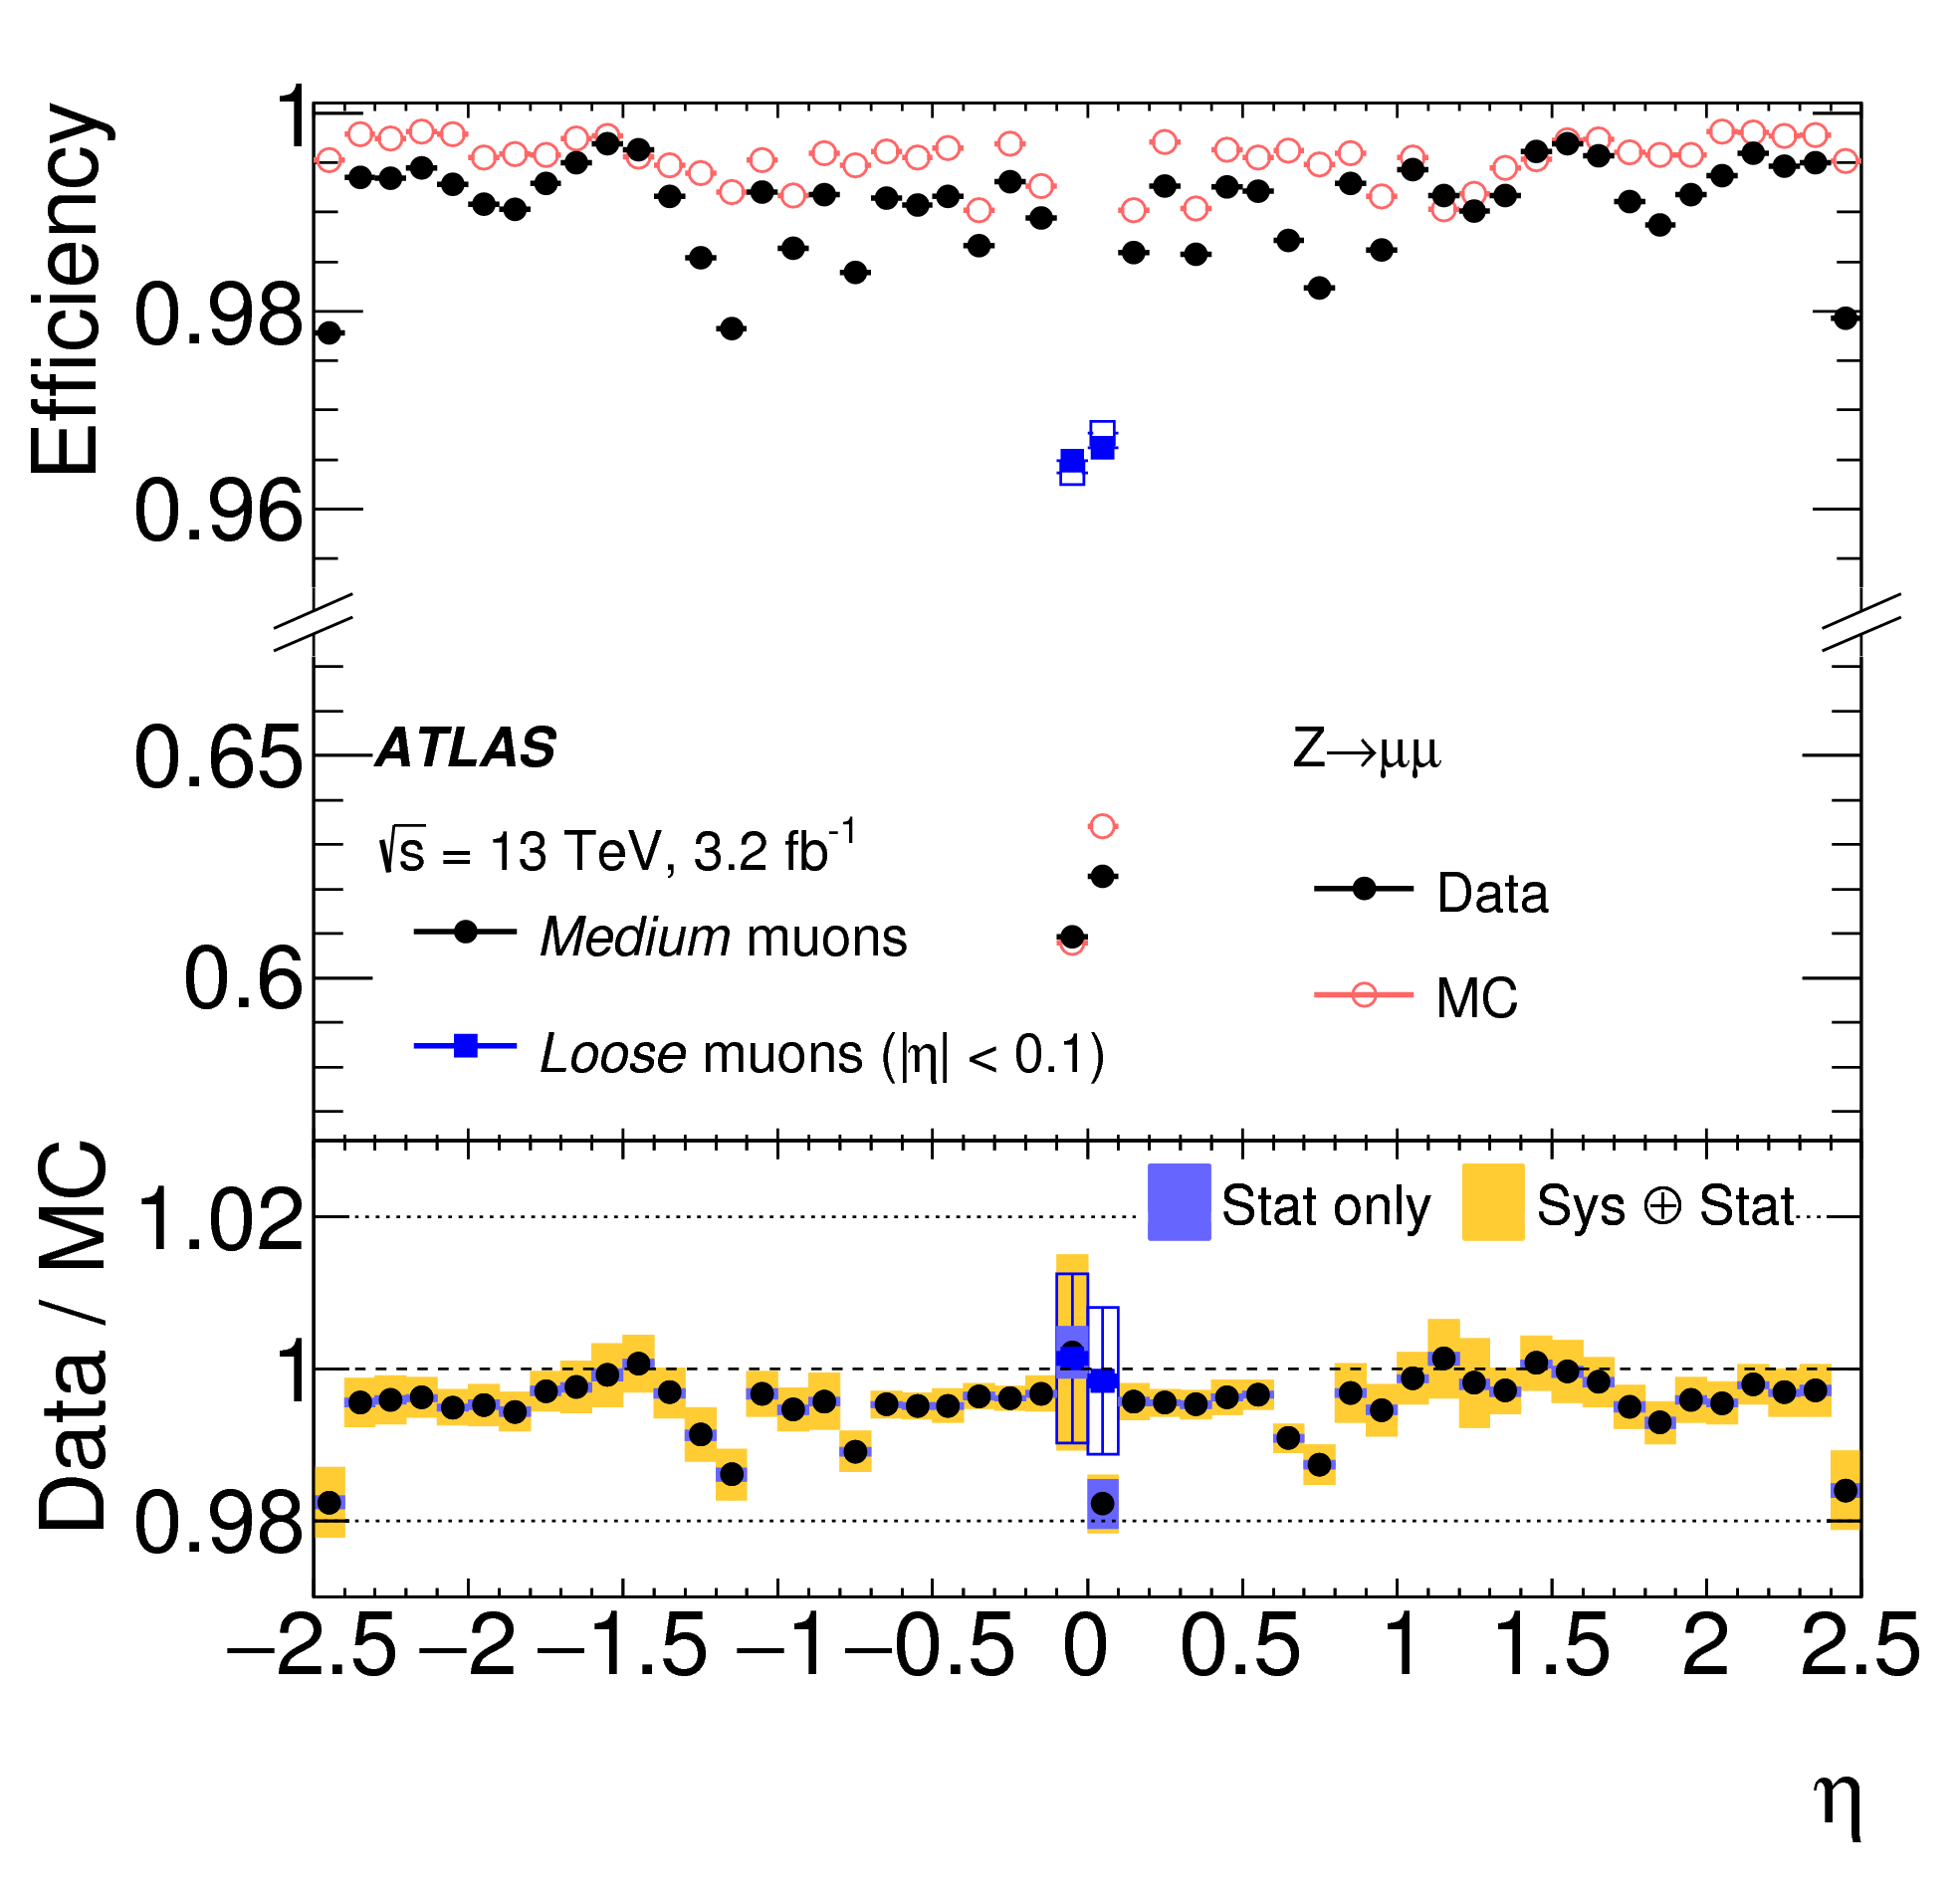
\includegraphics[width=.43\textwidth]{figures/EventReconstruction/muon-reco-eta.png}
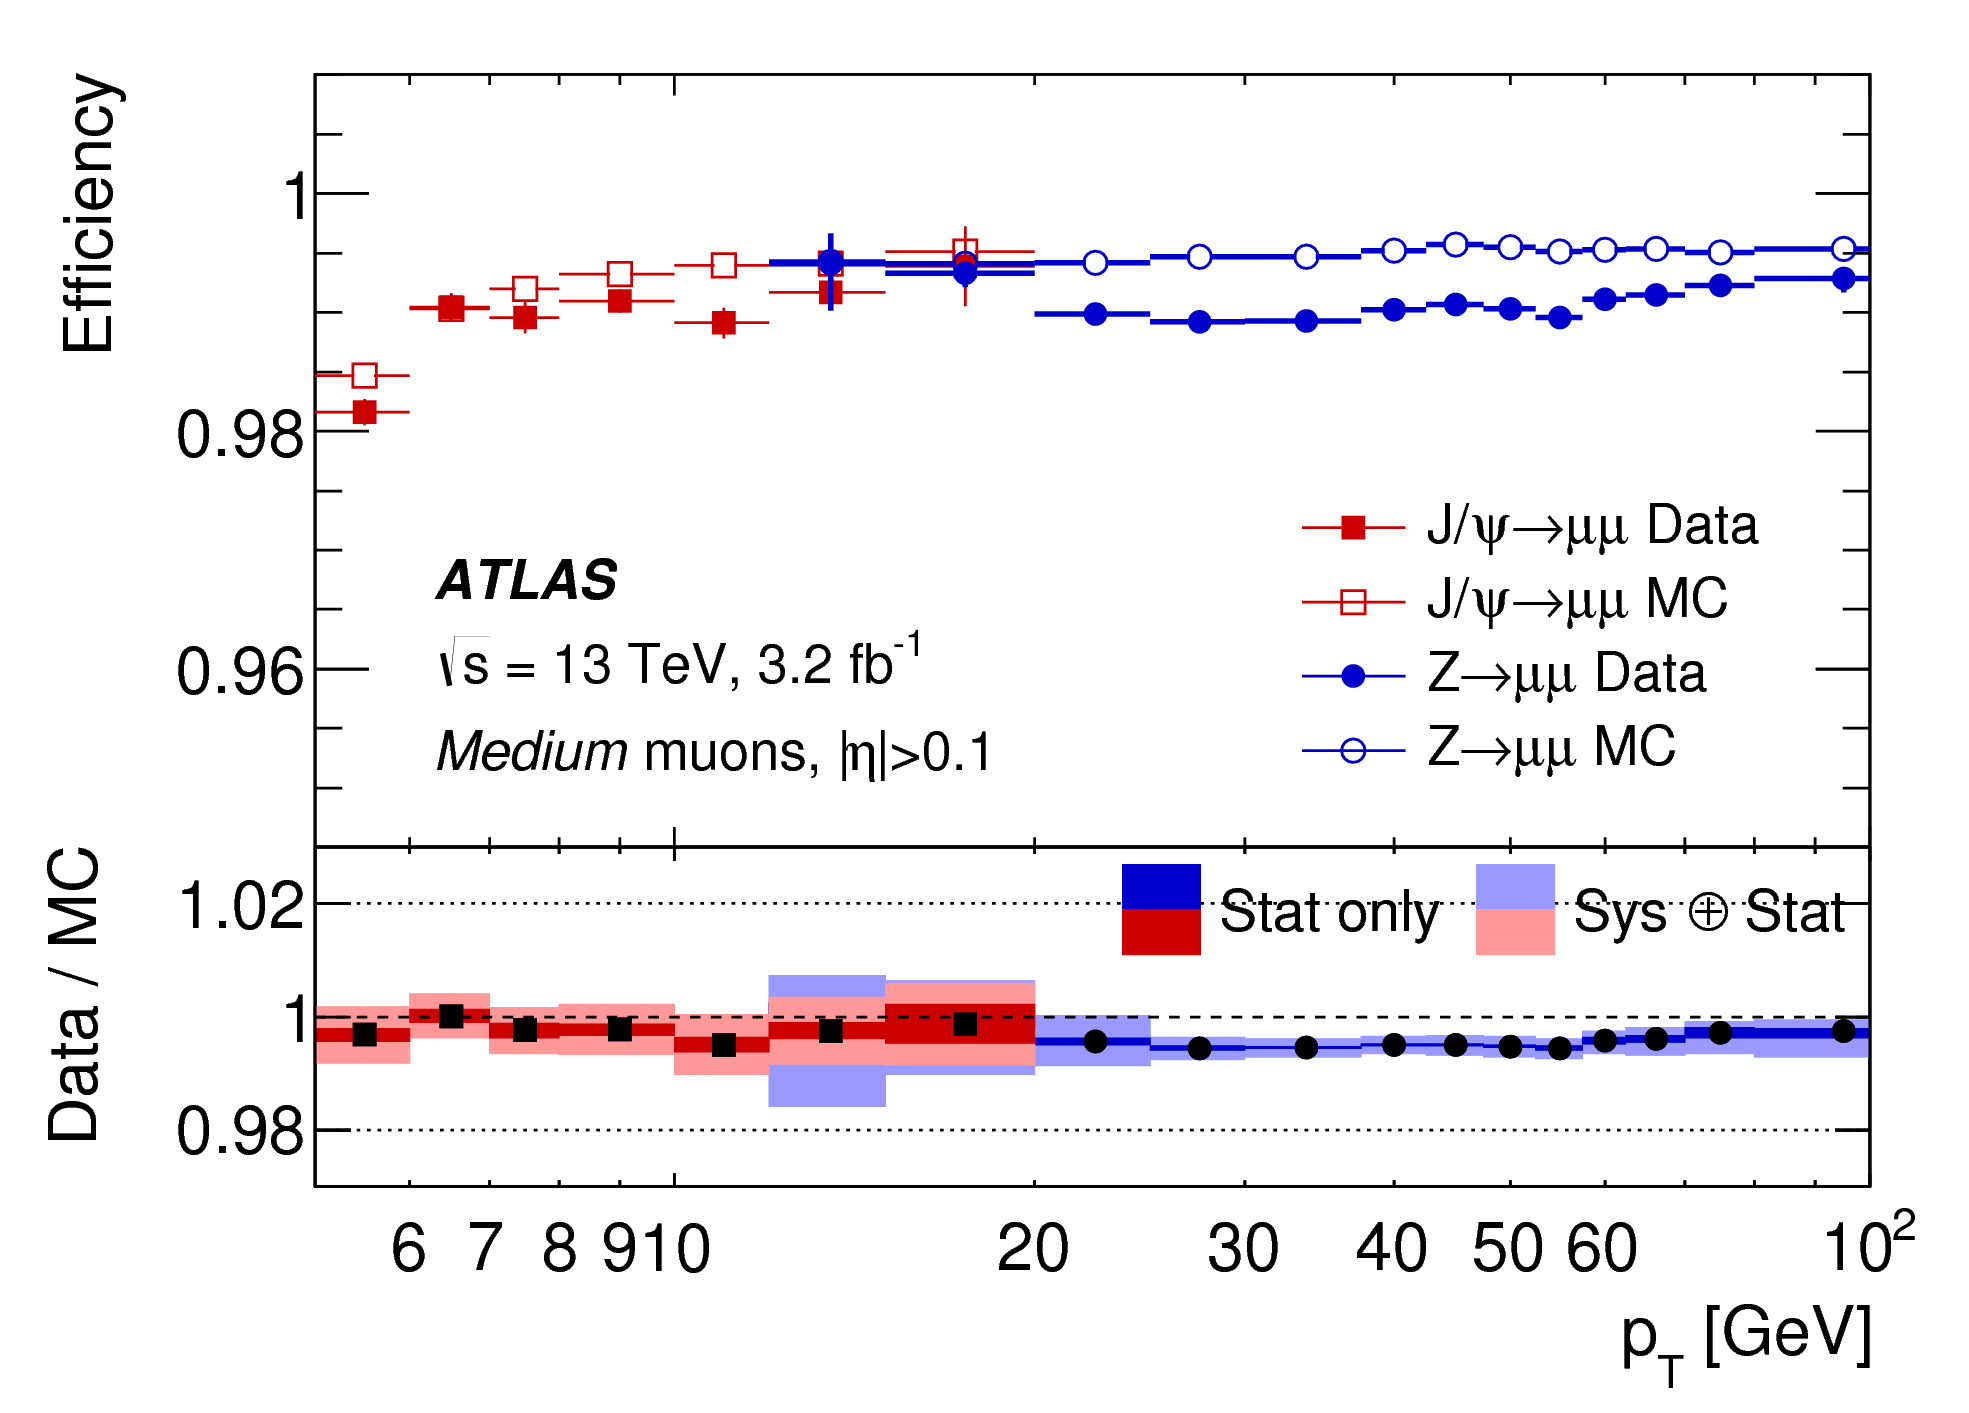
\includegraphics[width=.52\textwidth]{figures/EventReconstruction/muon-reco-pt.png}
\caption{Medium muon identification efficiency with standard tracking and criteria. Left is efficiency vs $\eta$ and right is efficiency as a function of $p_{T}$. Medium muons are reconstructed very efficiently, except for around $|\eta| \approx 0$, where the \ac{MS} is missing detector coverage.}
\label{fig:std_muon_eff}
\end{figure}


\subsection{Modifications}

For this analysis, muons are reconstructed after \ac{LRT} is performed and the reconstruction and identification efficiency is quite high. Furthermore, at the identification stage, we remove the requirement that the \ac{ID} track has at least one pixel hit, further improving the efficiency at high $d_{0}$. The effect of these improvements is show in \autoref{fig:cust_muon_eff}


This modification of the muon identification increases the fake rate of muons, so again we impose quality requirements that are independent of displacement. We require the muon to have at least two \ac{MS} layers with at least three precision hits, that the muon have at least one $\phi$ measurement (otherwise the \ac{MS} $\phi$ measurement is taken as the center of the \ac{MDT}, with an uncertainty of 0.2) and require the $\chi^{2}_{CB}/N_{DoF} < 3$. The $\chi^{2}_{CB}$ requirement is, in effect, a requirement on the consistency between the the \ac{ID} and \ac{MS} tracks. These will be further discussed in \autoref{sec:mu_qual_req}


\begin{figure}[htbp]
\centering
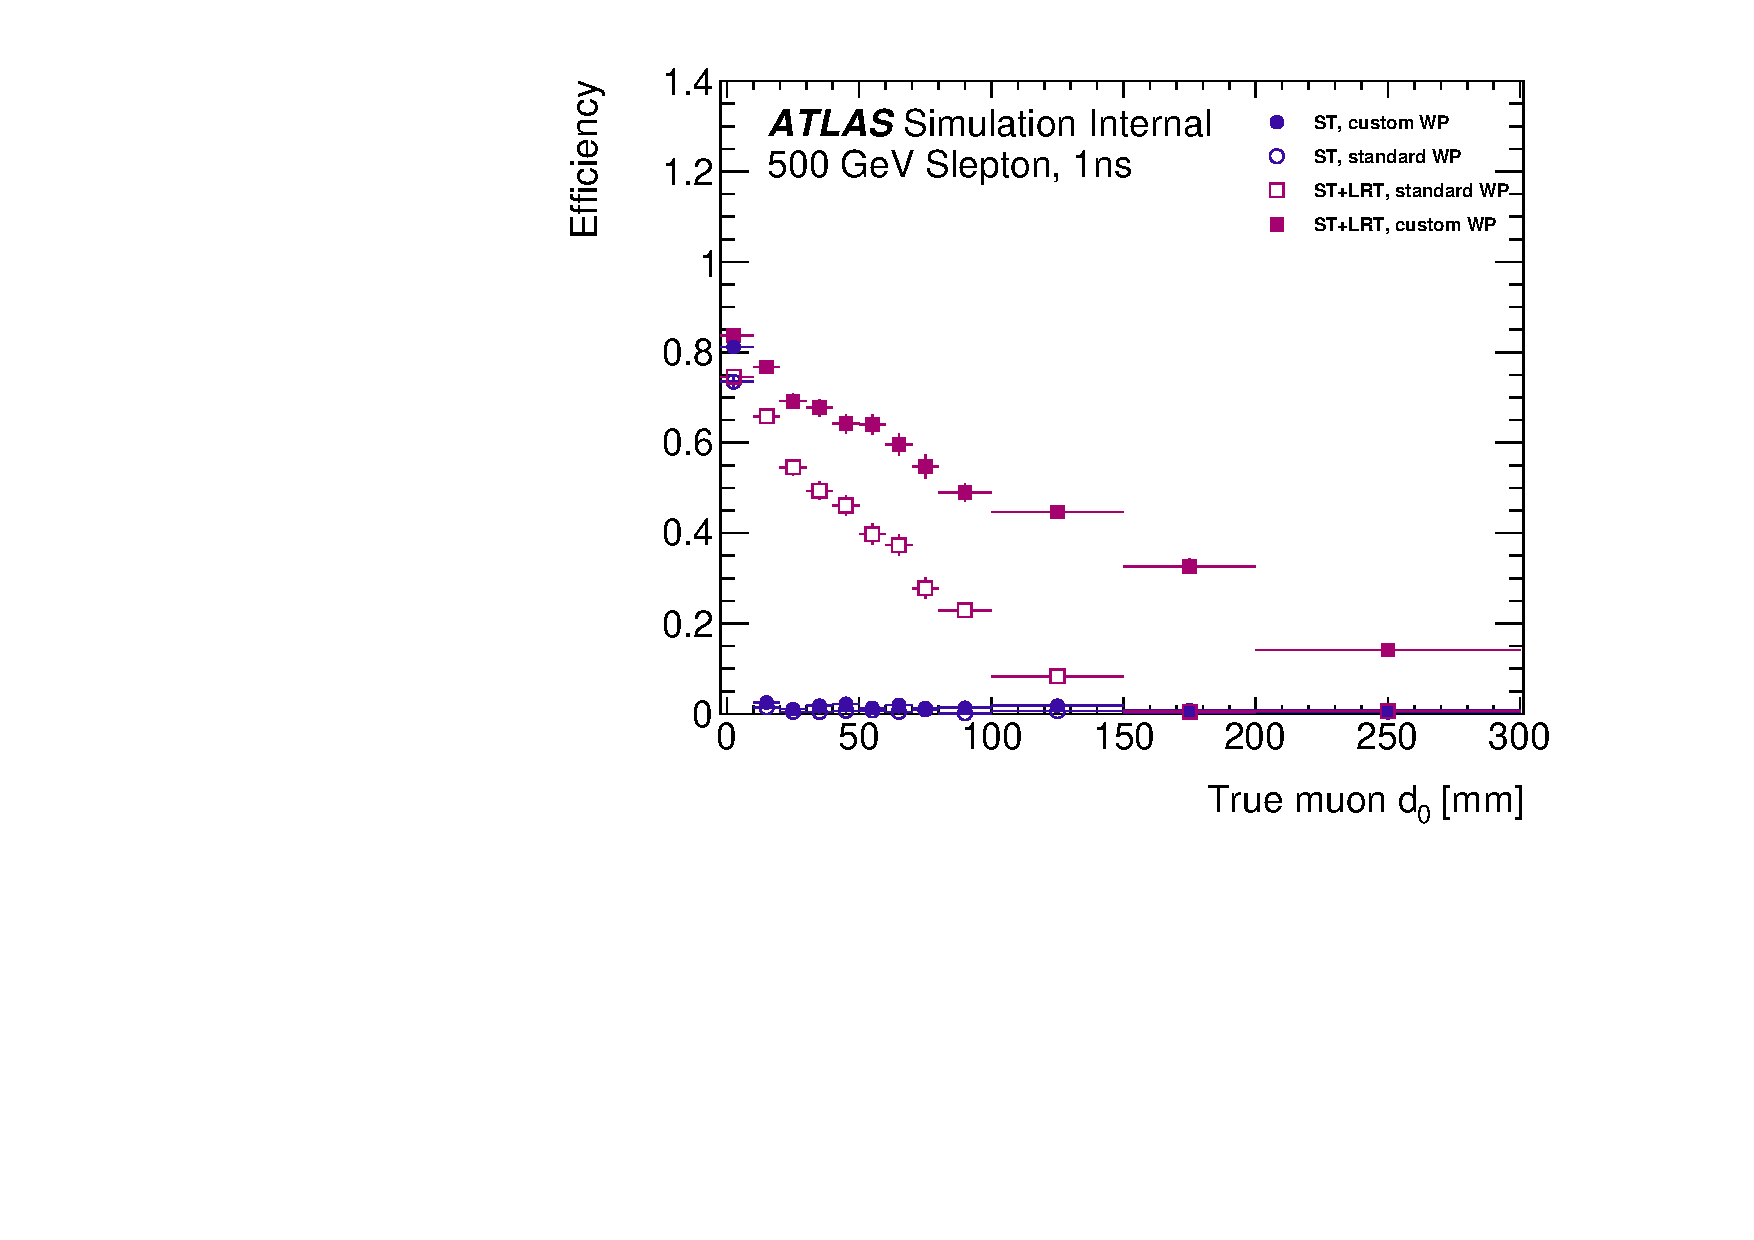
\includegraphics[width=.48\textwidth]{figures/EventReconstruction/wp_m_d0_all_wip.pdf}
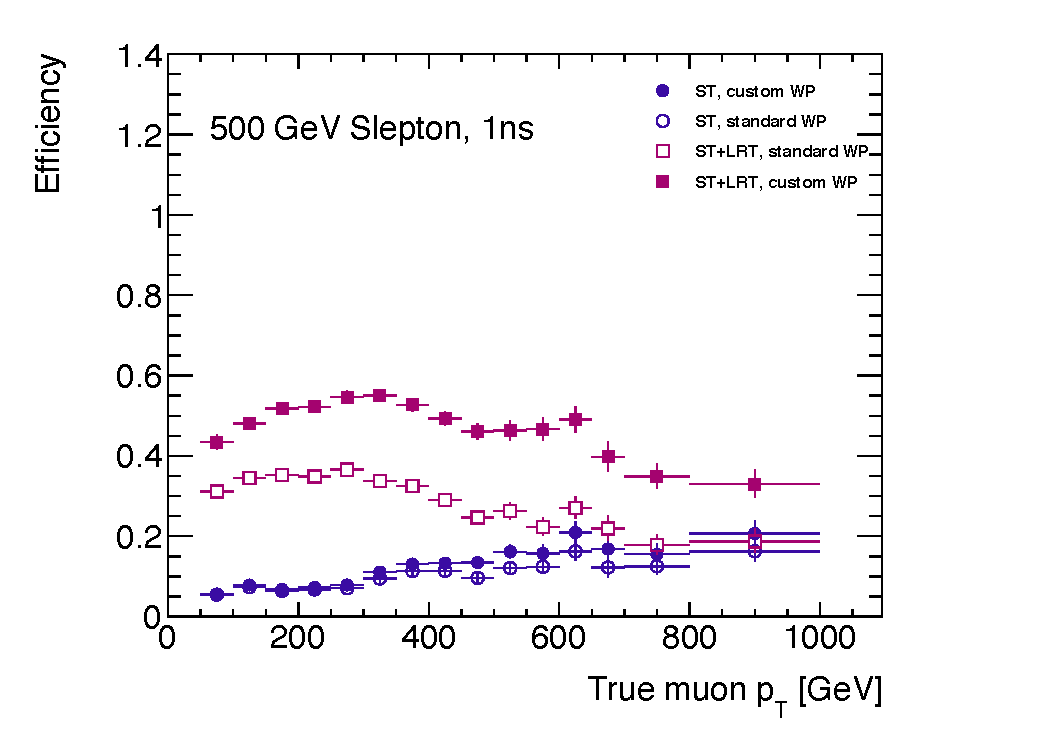
\includegraphics[width=.48\textwidth]{figures/EventReconstruction/wp_m_pt_all_wip.pdf}
\caption{Muon identification efficiency with modified criteria. Left is efficiency vs $d_{0}$ and right is efficiency as a function of $p_{T}$. The red denotes reconstruction with Standard Tracking (ST), and the blue with Large Radius Tracking (LRT), and the filled in circles use the modified identification working point. \todo{Needs update when available}}
\label{fig:cust_muon_eff}
\end{figure}



%-----------------------------
% Electron Reconstruction
%-----------------------------
\section{Electrons}
%USED atlas-electron-reco.pdf atlas-electron-reco-sliding-window.pdf
\label{sec:elecreco}

Electrons are reconstructed using clusters from the \ac{EM} calorimeter as well as tracks from the \ac{ID}. \cite{electron-reco} Electron reconstruction brings more complication and ambiguity than muon reconstruction because of the presence of photons, converted photons, and bremsstrahlung radiation from electrons moving through material. These factors make the identification and accurate measurement of electrons quite challenging. More than in muon reconstruction, it relies on displacement-based quality information, posing a problem for this search. We modify these requirements and use \ac{LRT} tracks, but have a resulting lower selection efficiency. 

\subsection{Standard Reconstruction and Identification}


\subsubsection{Cluster Reconstruction}

First, clusters are formed from $\eta \times \phi$ \emph{towers} of size $\Delta \eta \times \Delta \phi = 0.025 \times 0.025$ (roughly granularity of the second layer of the \ac{EM} calorimeter, where about 80\% of the energy in a shower is deposited). In each region, the energy deposited in all layers of the calorimeter is summed and are used as input to a seeding algorithm to form clusters. 

A \emph{sliding window} algorithm \cite{electron-sliding-window} is used to form clusters. In this algorithm, an $3 \times 5$ window is slid across each tower, the energy is summed inside of this window. If the sum is a local maximum and is above a threshold of $\et > 2.5 \GeV$, this window is considered a \emph{cluster}. A duplicate removal process is then performed for nearby clusters with similar energy measurements, keeping only the cluster with the largest $E_{T}$. Inefficiency in the cluster reconstruction step is negligible compared to the uncertainty in the next two steps. The efficiency of this step is 65\% at $\et = 4.5 \GeV$ and $> 99\%$ above $\et = 15 \GeV$.

\begin{figure}[htbp]
\centering
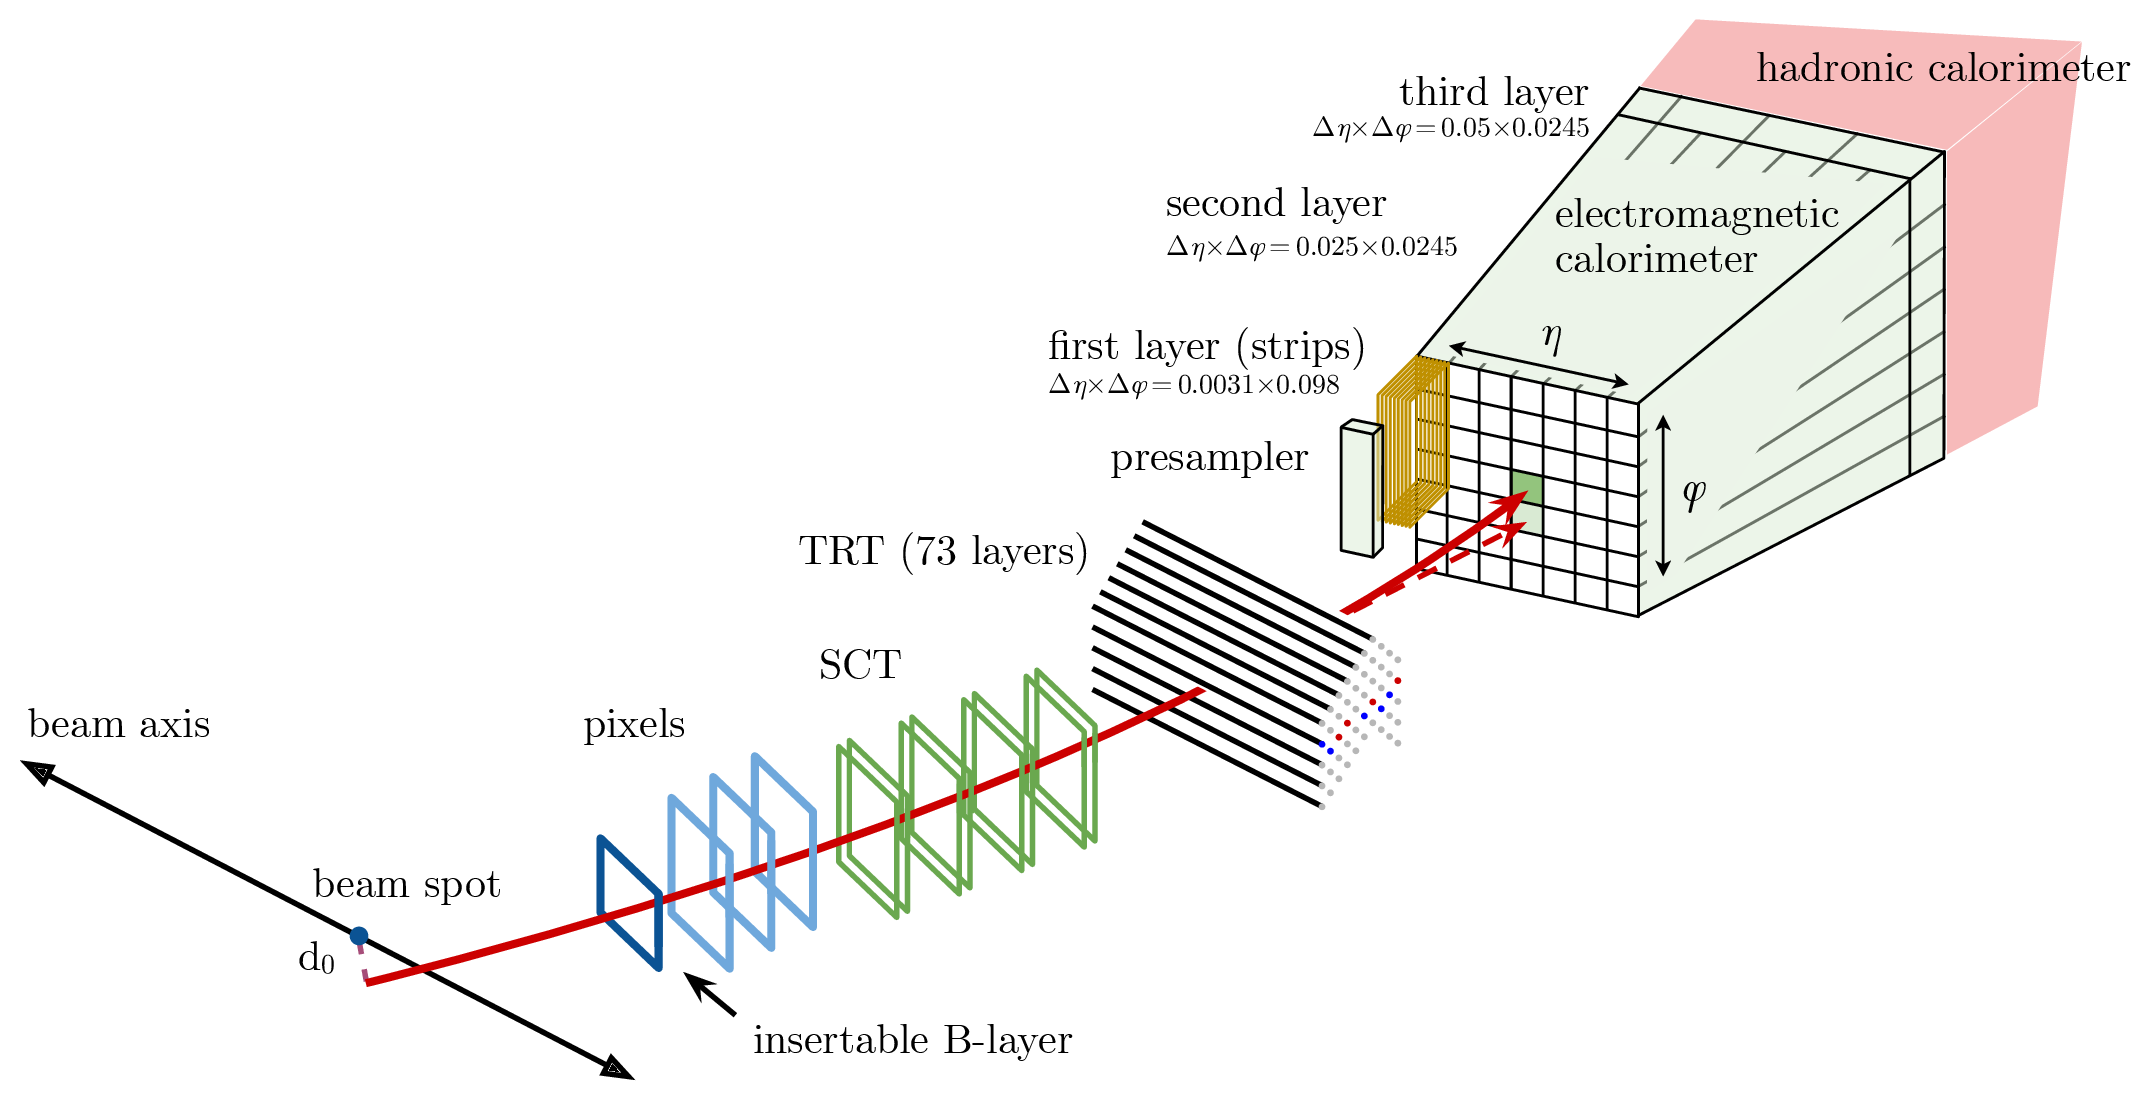
\includegraphics[width=.8\textwidth]{figures/EventReconstruction/electron-reco-sketch.png}
\caption{A sketch of an electron's path through a slice of the \ac{ATLAS} detector.}
\label{fig:elec_reco_sketch}
\end{figure}

\subsubsection{Tracking}
Since electrons are so light, they can lose a significant amount of their energy due to bremsstrahlung radiation as they traverse the \ac{ID}, thus resulting in a track seed that cannot be extended to the requisite number of silicon layers using the processes described in \autoref{sec:trackreco}. Thus, a second pass at tracking, allowing for 30\% energy loss due to bremsstrahlung radiation at each detector layer is performed in the vicinity of a good quality \ac{EM} cluster. Here, the track candidate $p_{T}$ is lowered to $400 \MeV$ (compare to $1 \GeV$), but still uses the standard hypothesis that the track is like that from a pion. If this fit still fails, a third pass is performed using the assumption that the track is like that from an electron, allowing for an additional degree of freedom in the $\chi^2$ calculation that accounts for additional radiation. In all, this gives 98\% reconstruction efficiency for electrons with $\et > 10 \GeV$. 

This loosened track fitting requirements allow for increased efficiency, but the resulting tracks do not correctly account for the energy loss of the electron to the material. An additional tracking pass, using an optimized \ac{GSF} is used to correct for this. 

This procedure is performed on tracks with at least 5 silicon hits and roughly match to an \ac{EM} cluster. The \ac{GSF} procedure is based on a combinatorial Kalman filter, resulting in track parameters weighted by Gaussian function describing material-induced energy losses. This procedure also accounts for the increase in curvature caused by the decrease in momentum due to energy loss in material, improving the calculation of track parameters. An example of this is show in the figure below. The reconstruction efficiency for this step is around 98\% for electrons with $\et > 30 \GeV$. 

\begin{figure}[htbp]
\centering
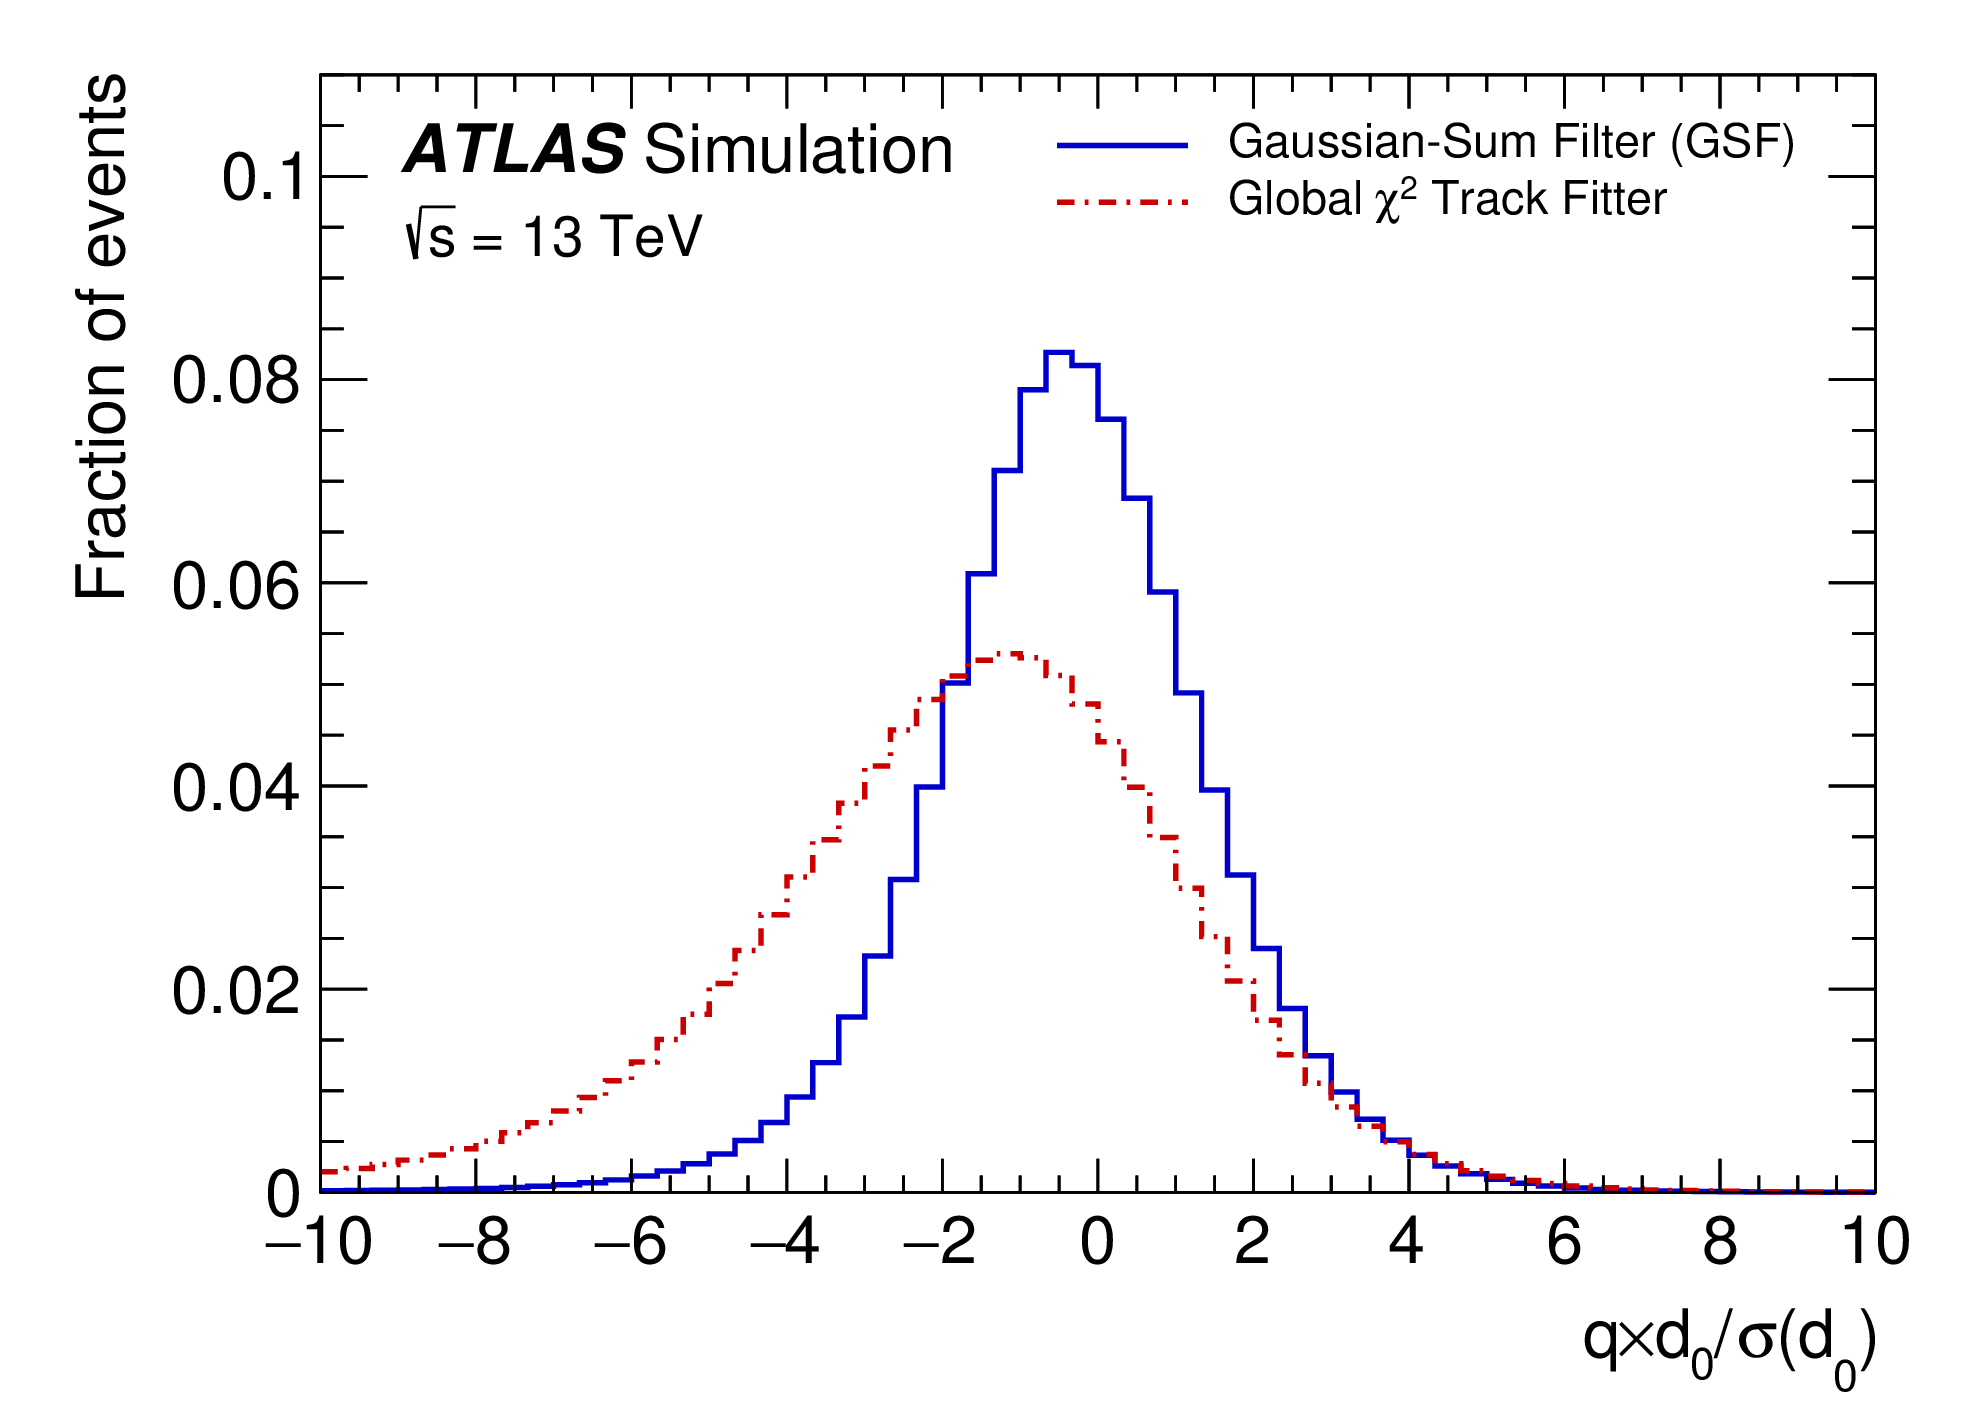
\includegraphics[width=.7\textwidth]{figures/EventReconstruction/elec-qxd0.png}
\caption{The impact on the $q \times \dzero /\sigma(\dzero)$ measurement by the addition of \ac{GSF} tracking. This is sampled from prompt electrons, so the narrower distribution centered around zero indicates significant improvement.}
\label{fig:elec_gsf}
\end{figure}


\subsubsection{Combined Reconstruction}
To put it all together, \ac{GSF} tracks are then matched to seed calorimeter clusters then the final cluster size is determined. Tracks and clusters are matched with stricter requirements, requiring that their $\phi$ measurement is within $+0.05$ or $-0.10$. It is possible that several tracks might match to the same cluster, but a primary track is assigned based on its proximity and quality. If the track can be associated to a vertex, it is classified as a potential photon conversion, not an electron. Electrons are further distinguished from photon conversions using their $E/p, p_{T}$, and number of pixel hits. 

Final clusters are formed by looking in a window around the seed cluster. The reconstructed electron's energy measurement is taken from its full cluster, and directional information taken from its track. At $\et > 15 \GeV$, there is a 99\% efficiency to reconstruct an electron (provided it has at least one pixel hit and at least seven total silicon hits on track). 

\begin{figure}[htbp]
\centering
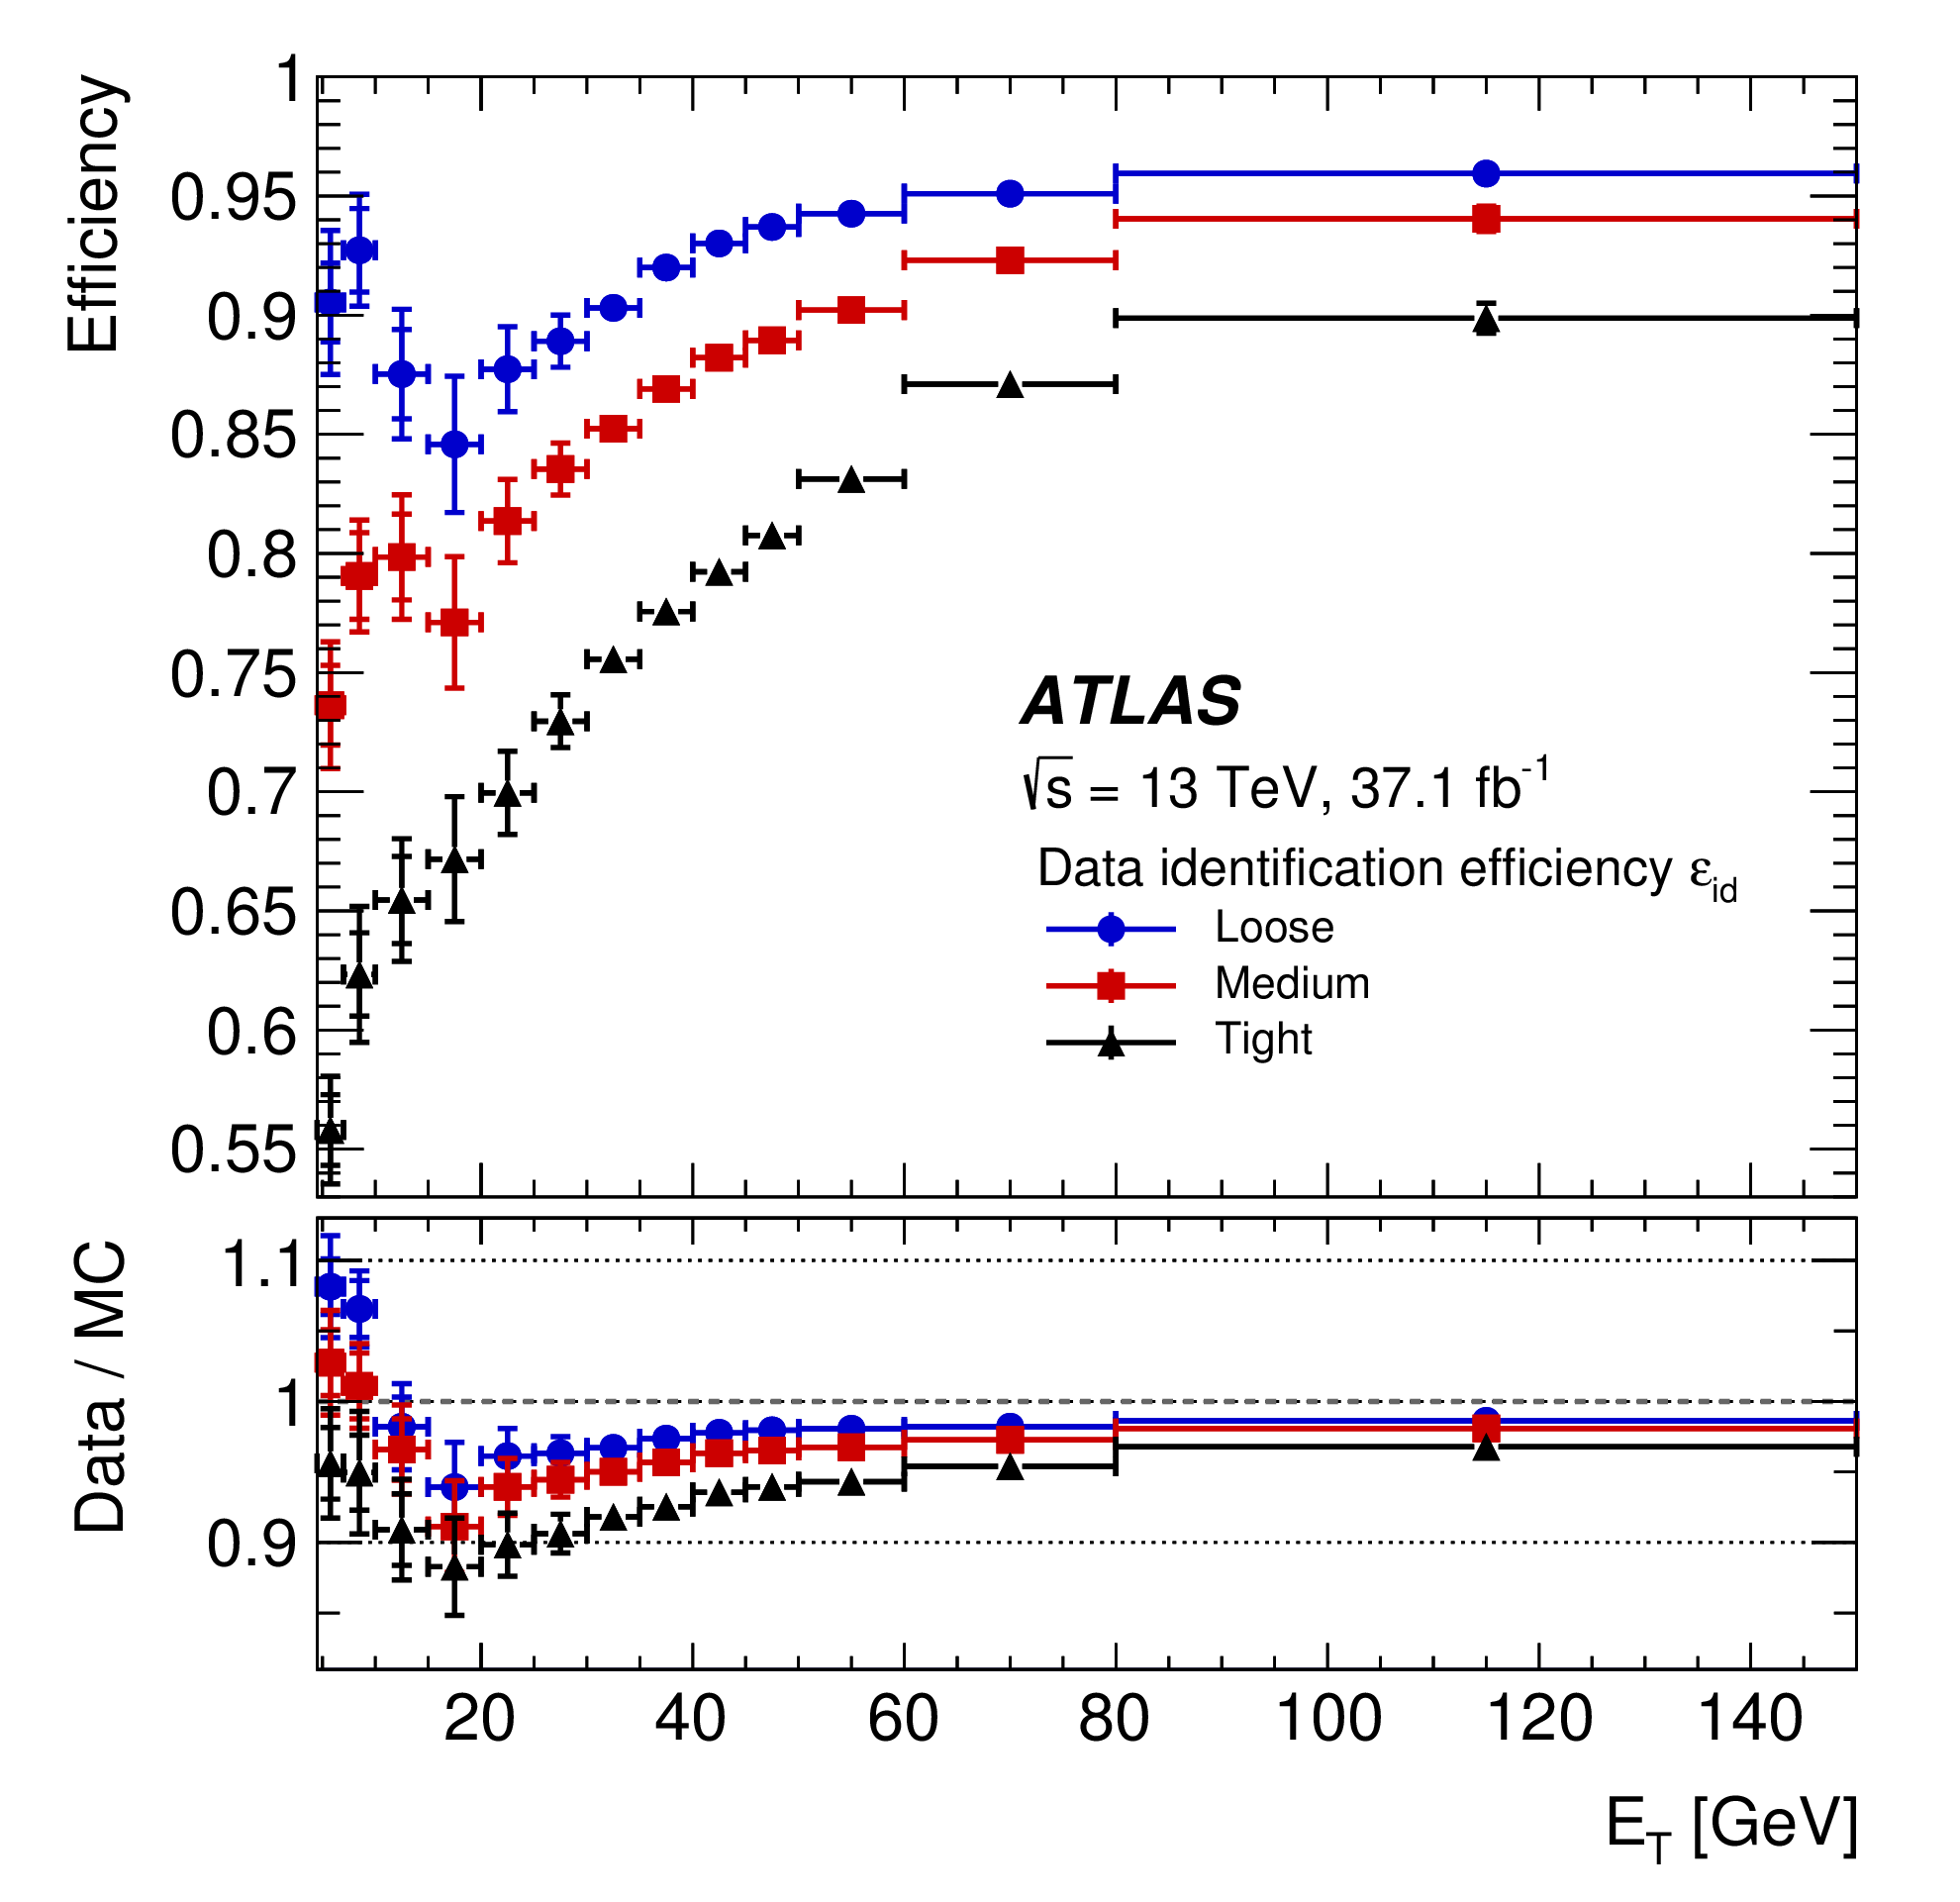
\includegraphics[width=.4\textwidth]{figures/EventReconstruction/elec-reco.png}
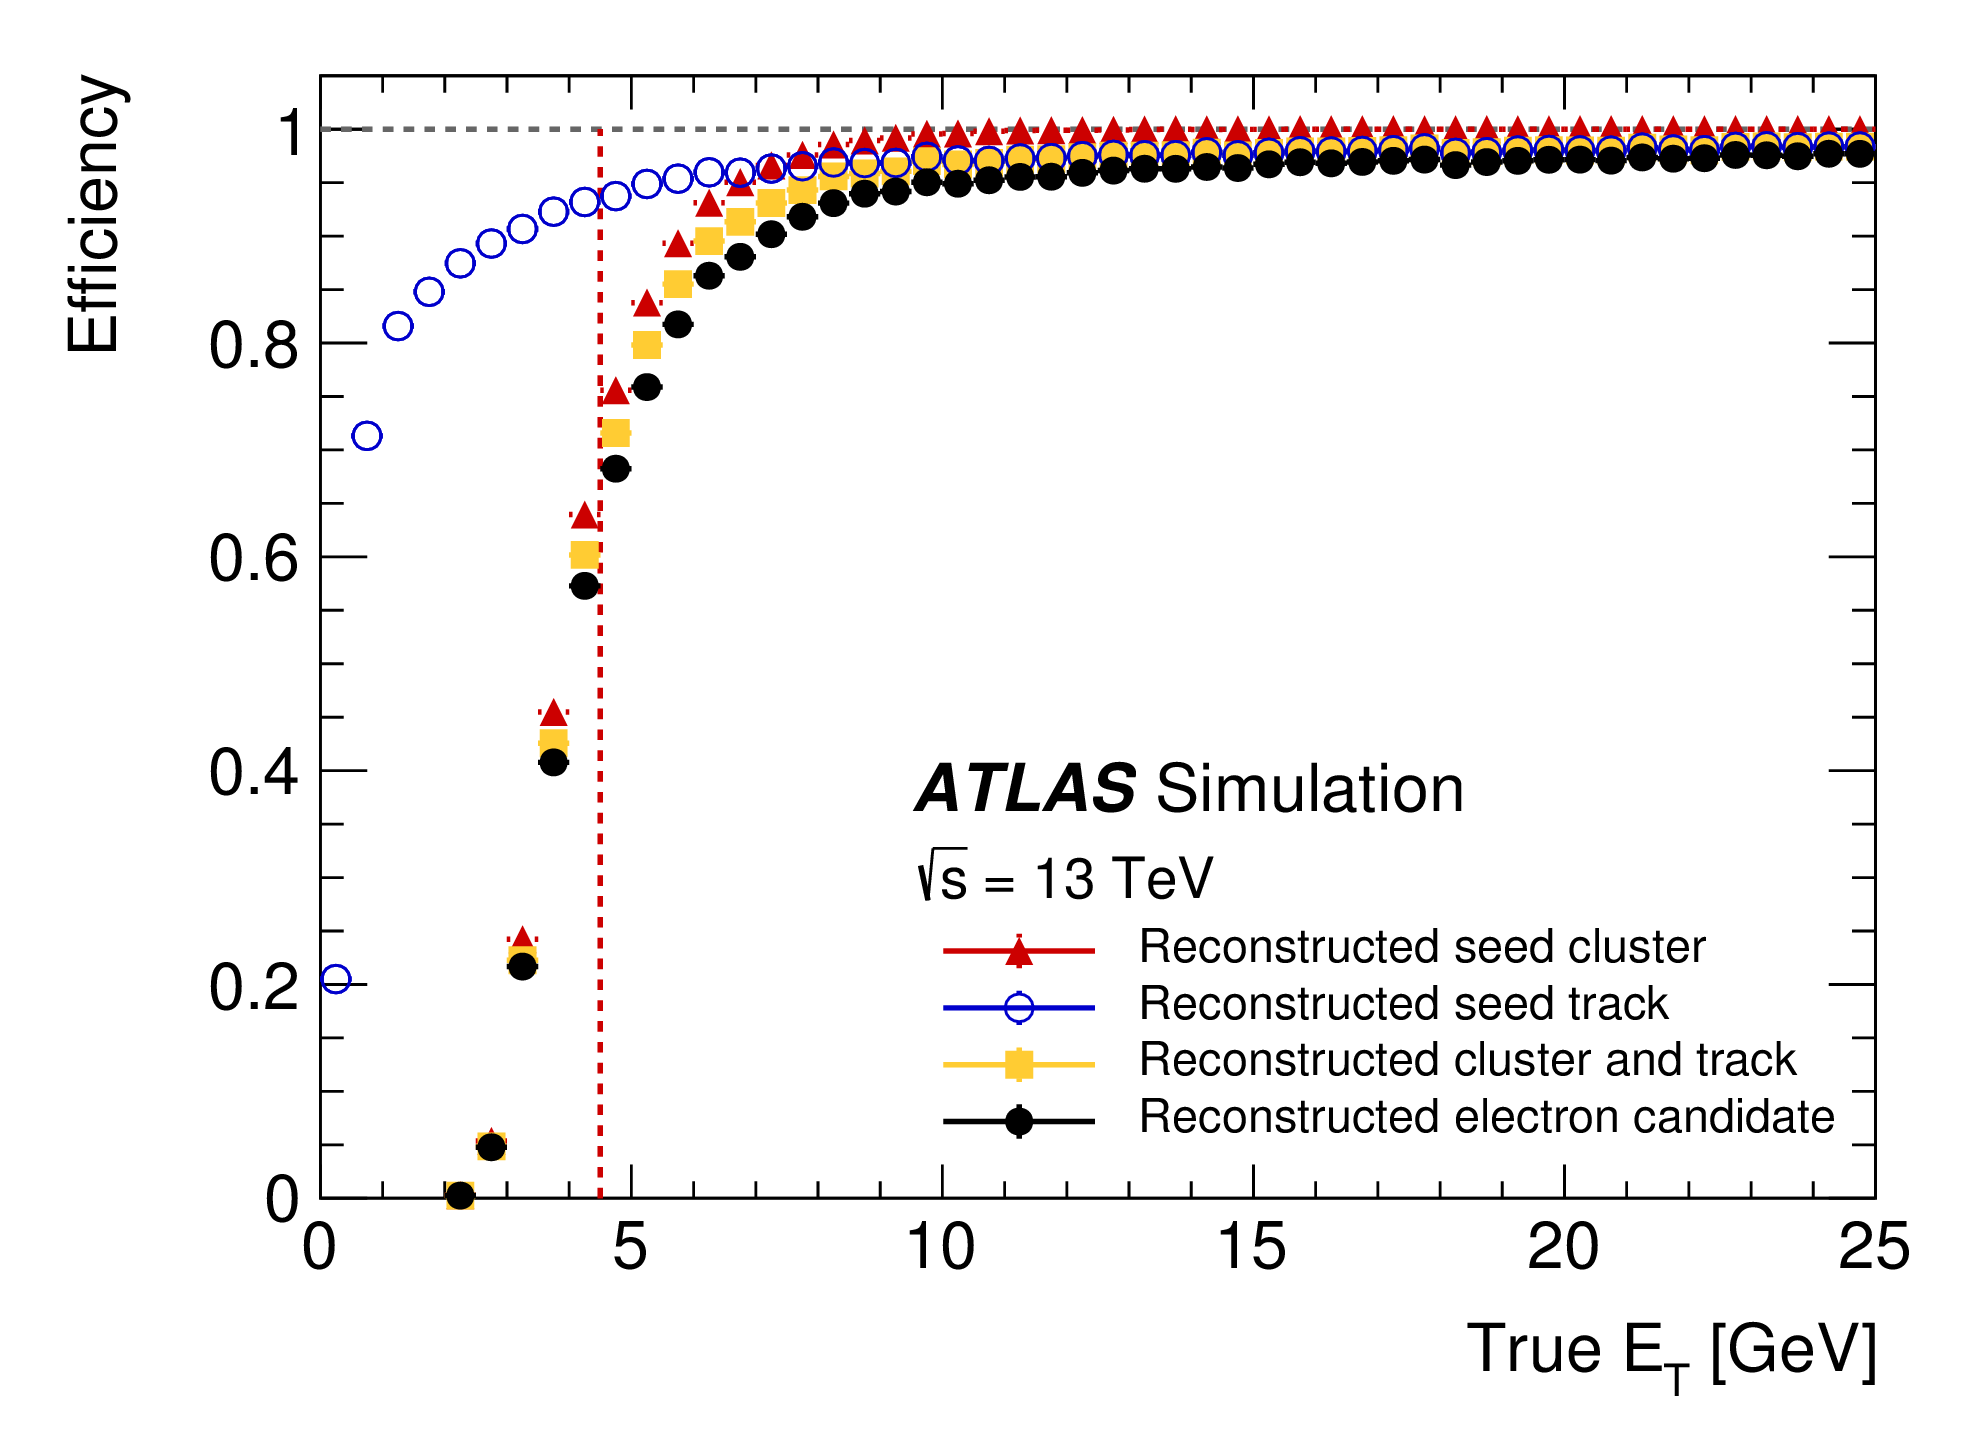
\includegraphics[width=.5\textwidth]{figures/EventReconstruction/elec-reco-steps.png}
\caption{Electron reconstruction efficiency as a function of true transverse energy, \et. For the various electron working points (left) and for each step in the reconstruction process (right).}
\label{fig:elec_gsf}
\end{figure}

\subsubsection{Identification}

Electrons are identified using a likelihood that further distinguishes them from photons, light flavor jets, and leptonic heavy flavor decays. The likelihood is more flexible than a simple cut-based method, allowing for electrons to fail one selection criterion. It also allows for the use of discriminating criteria which have relatively similar shapes in signal and background. A some cuts are made at the identification step, including on the number of pixel and silicon hits, as well as on the shower width. Many other factors not cut on but are included in the likelihood including the track quality, consistency between the electron's track and its cluster, as well energy ratios in the various layers of the \ac{EM} calorimeter, as well as the \ac{EM} calorimeter compared to the hadronic calorimeter.


\subsection{Modifications}
To be able to reconstruct electrons with high impact parameter, several changes needed to be made to the reconstruction and identification algorithms. 

Similar to the muon case, the reconstruction is then run on the track collection including \ac{LRT} tracks. At the identification stage, we remove variables concerned with $d_{0}$ from the likelihood consideration, but do not retrain the likelihood itself. We also remove the cut on the number of silicon hits on top of that made at the reconstruction stage. 

After these modifications, we introduce many fake electrons, primarily resulting from a fake \ac{LRT} track being associated to an \ac{EM} cluster from a photon. The most powerful discriminator is the consistency in the $p_{T}$ as measured by the track and the cluster, defined as $\Delta p_{T} = p_{T}^{track}/p_{T}^{e}$. Furthermore, we require the primary track to be good quality, with $\chi^{2} < 2$ and at maximum one missing hit on track after the innermost hit. These will be further discussed in \autoref{sec:elec_qual_req}

\begin{figure}[htbp]
\centering
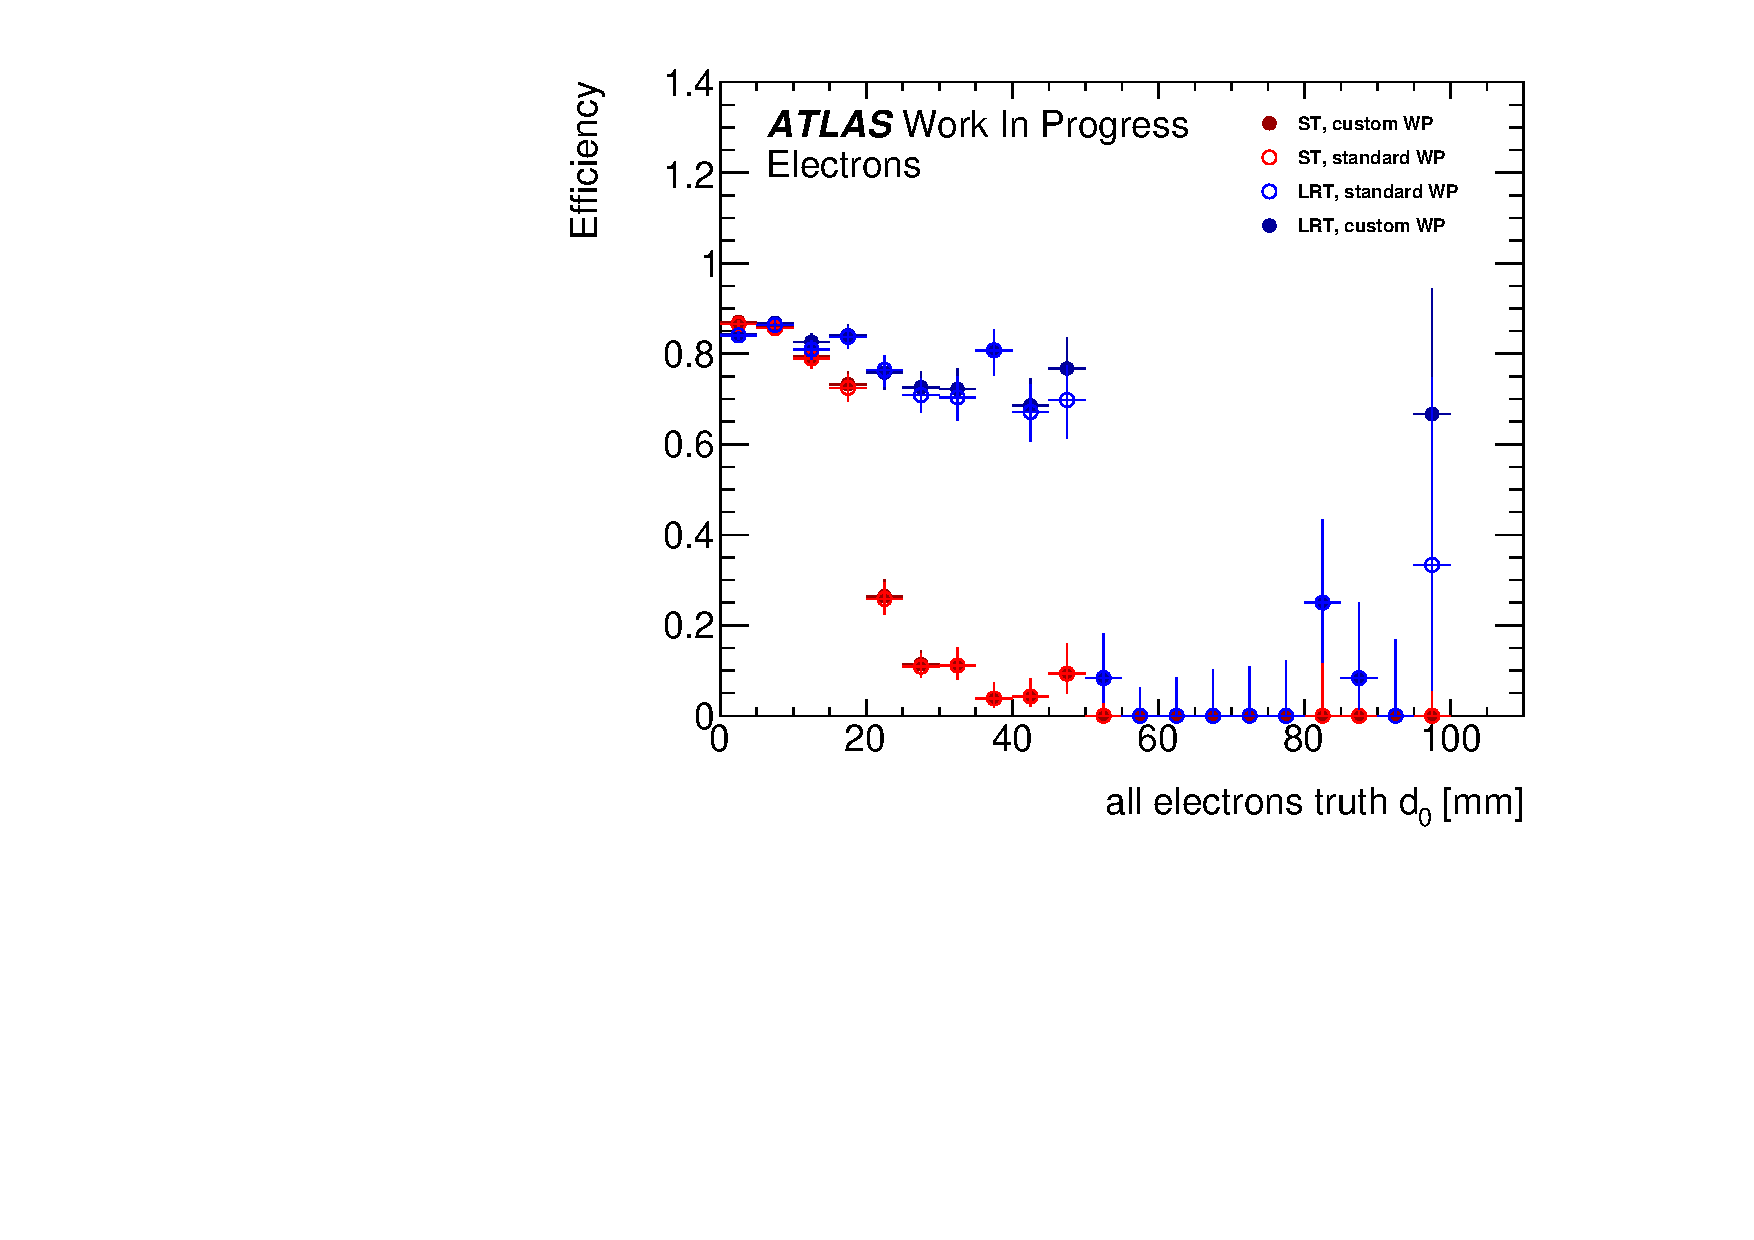
\includegraphics[width=.48\textwidth]{figures/EventReconstruction/wp_e_d0_all_wip.pdf}
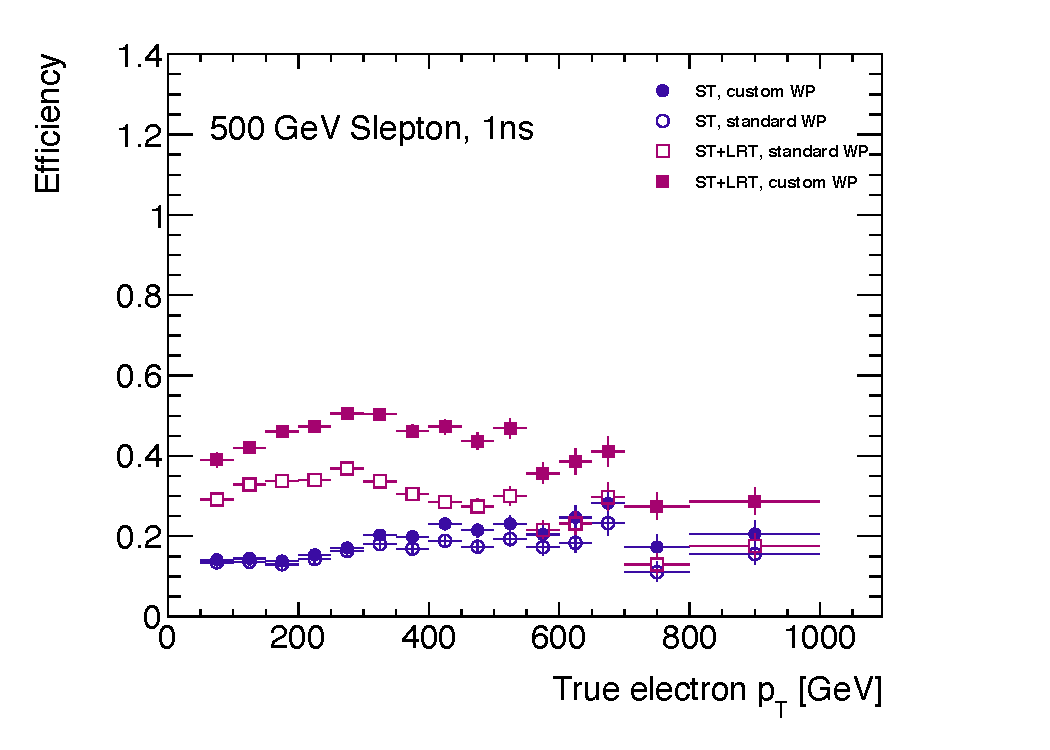
\includegraphics[width=.48\textwidth]{figures/EventReconstruction/wp_e_pt_all_wip.pdf}
\caption{Muon identification efficiency with modified criteria. Left is efficiency vs $d_{0}$ and right is efficiency as a function of $p_{T}$. The red denotes reconstruction with Standard Tracking (ST), and the blue with Large Radius Tracking (LRT), and the filled in circles use the modified identification working point. \todo{Needs update when available}}
\label{fig:cust_elec_eff}
\end{figure}




\section{Isolation}

In this analysis, both muons and electrons are required to be isolated to reduce background from heavy flavor decays. That is, they are not expected to be surrounded by much other activity from the hard scatter in either the Inner Detector or Calorimeters. Isolation is generally measured in terms as the scalar sum of energy in a radius $\Delta R = \sqrt{(\Delta \eta)^2 + (\Delta \phi)^2}$ around the lepton. Track based isolations are called $p_{T}^{\textrm{varcone}}$ and calorimeter based isolations called $E_{T}^{\textrm{topocone}}$. 

For example, the track-based isolation called $p_{T}^{\textrm{varcone30}}$ is the scalar sum of the transverse momenta of tracks with $p_{T} > 1 \GeV$ in a cone of $\Delta R = \textrm{min}(10 \GeV/p_{T}^{\ell}, 0.3)$, then a value is selected to determine what should be considered ``isolated''. Whereas the calorimeter-based isolation just counts the energy in a specified \dR, not as a function of the \pt of the particle. Isolation working points are then centrally defined as a combination of cuts on the track-based and calorimeter-based isolation. 

These definitions are much simpler for muons than for electrons. Electrons are very likely to emit bremsstrahlung radiation as they traverse the inner detector and those photons can then convert back into electrons. The tracks from these secondary particles are considered part of the electron's \pT. Furthermore, the electron leaves its own energy deposit in the \ac{EM} calorimeter and this energy must be subtracted from the $E_{T}^{\textrm{topocone}}$ calculation.


In this analysis we use the following working points \todo{grab isolation requirements from INT when finalized}



